%% LyX 2.0.6 created this file.  For more info, see http://www.lyx.org/.
%% Do not edit unless you really know what you are doing.
\documentclass[11pt,polish,pdflatex]{aghdpl}
\usepackage[T1]{fontenc}
\usepackage[latin2]{inputenc}
\usepackage{listings}
\usepackage{textcomp}
\usepackage{amssymb}
\usepackage{graphicx}
\usepackage{setspace}
\usepackage{subscript}

\makeatletter

%%%%%%%%%%%%%%%%%%%%%%%%%%%%%% LyX specific LaTeX commands.
%% Because html converters don't know tabularnewline
\providecommand{\tabularnewline}{\\}

%%%%%%%%%%%%%%%%%%%%%%%%%%%%%% User specified LaTeX commands.

% \documentclass{aghdpl}               % przy kompilacji programem latex
% \documentclass[pdflatex,en]{aghdpl}  % praca w j�zyku angielskim



% dodatkowe pakiety
\usepackage{enumerate}
\usepackage{listings}
\lstloadlanguages{TeX}

%---------------------------------------------------------------------------

\author{Marcin Szpyrka}
\shortauthor{M. Szpyrka}

\titlePL{Przygotowanie pracy dyplomowej w~systemie \LaTeX}
\titleEN{Thesis in \LaTeX}

\shorttitlePL{Przygotowanie pracy dyplomowej w~systemie \LaTeX} % skr�cona wersja tytu�u je�li jest bardzo d�ugi
\shorttitleEN{Thesis in \LaTeX}

\thesistypePL{Praca magisterska}
\thesistypeEN{Master of Science Thesis}

\supervisorPL{dr hab. Marcin Szpyrka}
\supervisorEN{Marcin Szpyrka Ph.D}

\date{2009}

\facultyPL{Wydzia� Elektrotechniki, Automatyki, Informatyki i Elektroniki}
\facultyEN{Faculty of Electrical Engineering, Automatics, Computer Science and Electronics}

\acknowledgements{Serdecznie dzi�kuj� \dots tu ci�g dalszych podzi�kowa� np. dla promotora, �ony, s�siada itp.}

%---------------------------------------------------------------------------

\makeatother

\usepackage{babel}
\begin{document}
\author{�ukasz Cisowski\\Pawe� Mazik}
\shortauthor{�. Cisowski, P. Mazik}

\titlePL{Pozycjometr inercyjny}
\titleEN{Inertial position meter}

\shorttitlePL{Pozycjometr inercyjny}
\shorttitleEN{Inertial position meter}

\thesistypePL{Praca in�ynierska}
\thesistypeEN{Bachelor's Thesis}

\supervisorPL{dr in�. Krzysztof �wientek}
\supervisorEN{Dr Eng. Krzysztof �wientek}
\acknowledgements{Serdecznie dzi�kujemy promotorowi za pomoc i nieocenione uwagi, kt�re przyczyni�y si� do znacznej poprawy merytorycznej pracy.} 

\facultyPL{Wydzia� Fizyki i Informatyki Stosowanej}
\facultyEN{Faculty of Physics and Applied Computer Science}

\departmentPL{Katedra Oddzia�ywa� i Detekcji Cz�stek}
\departmentEN{Department of Particle Interaction and Detection Techniques}

\date{2015}

\titlepages   

\tableofcontents{}\clearpage{}


\chapter{Wprowadzenie\label{cha:wprowadzenie}}

W dzisiejszych czasach, ze wzgl�du na szerokie rozpowszechnienie smartfon�w,
w zasadzie ka�dy z nas ma kontakt (�wiadomy b�d� nie�wiadomy) z uk�adami
mierz�cymi po�o�enie urz�dzenia w przestrzeni. Akcelerometry i �yroskopy
stanowi� wyposa�enie wielu nowoczesnych urz�dze�, pozwalaj�c zwi�kszy�
ich komfort u�ytkowania. 

Akcelerometr pozwala na korzystanie z urz�dze� dotykowych niezale�nie
od ich po�o�enia. Dzi�ki niemu mo�liwe jest ,,obr�cenie'' zawarto�ci
ekranu wraz ze zmian� orientacji urz�dzenia w przestrzeni. �yroskop
wykorzystywany jest przyk�adowo w grach, w kt�rych kontrola sprawowana
jest za pomoc� zmiany k�ta po�o�enia telefonu wzgl�dem poziomu (np.
w grach wy�cigowych). Tak wi�c ka�dego dnia u�ywamy pozycjometru wbudowanego
w smartfon, nie zawsze zdaj�c sobie sprawy z jego obecno�ci.

Oczywi�cie wykorzystanie akcelerometr�w i �yroskop�w nie ogranicza
si� jedynie do ich zastosowa� w urz�dzeniach mobilnych. Czujniki przy�pieszenia
wykorzystywane s� r�wnie� np. w uk�adach stabilizacji optycznej, zabezpieczeniach
chroni�cych przed skutkami upadk�w, uk�adach automatyki i~robotyki,
jako detektory ruchu i zderze�. �yroskopy wykorzystuje si� g��wnie
w uk�adach pomiarowych k�t�w obrotu, oscylatorach, uk�adach regulacji
amplitudy drga� czy te� w demodulatorach synchronicznych. Du�a ilo�ci�
akcelerometr�w i �yroskop�w, wykorzystuj�cych w swoim dzia�aniu r�ne
zjawiska fizyczne i ich znaczna rozpi�to�� cenowa sprawi�y, �e urz�dzenia
te sta�y si� bardzo popularne i powszechnie wykorzystywane w technice.

Przedmiotem niniejszej pracy jest zrealizowanie pozycjometru inercyjnego
na mikroprocesorze ARM CortexM3 z wykorzystaniem akcelerometru i �yroskopu
wykonanych w technologii MEMS (\emph{Micro Electro-Mechanical Systems})
- wykonanych w krzemie uk�ad�w elektro-mechanicznych. Ze wzgl�du na
fakt, i� jest to praca wykonywana wsp�lnie przez dwie osoby, dokonano
nast�puj�cego podzia�u zada� koniecznych do wykonania:
\begin{itemize}
\item �ukasz Cisowski -- komunikacja mikroprocesora z urz�dzeniami pomiarowymi,
dokonanie pomiaru, przetworzenie wynik�w;
\item Pawe� Mazik -- przygotowanie p�ytki koniecznej do po��czenia mikrokontrolera
z uk�adami pomiarowymi, komunikacja z komputerem, interfejs u�ytkownika.
\end{itemize}
Je�li za� chodzi o niniejsz� prac�, to poszczeg�lne rozdzia�y zosta�y
napisane wg nast�puj�cego podzia�u:
\begin{itemize}
\item �ukasz Cisowski -- rozdzia�y 2, 4, 6.2, 7.4;
\item Pawe� Mazik -- rozdzia�y 3, 5, 6.1, 6.3, 7.1, 7.2, 7.3, 7.5.\end{itemize}




\chapter{Akcelerometry}

\begin{onehalfspace}
Akcelerometr, zwany tak�e przy�pieszeniomierzem, jest czujnikiem s�u��cym
do pomiar�w przyspiesze� liniowych oraz k�towych. Przyspieszenie liniowe
jest wielko�ci� fizyczn�, okre�lon� nast�puj�cym wzorem:

\begin{equation}
\mathbf{a}=\frac{d\mathbf{v}}{dt}\label{eq:przyspieszenie_wzor_ogolny}
\end{equation}


gdzie:
\end{onehalfspace}
\begin{itemize}
\begin{onehalfspace}
\item \textbf{a} - wektor przyspieszenia,
\item \textbf{v} - wektor pr�dko�ci,
\item t - czas.\end{onehalfspace}

\end{itemize}
Rozk�adaj�c wektor \textbf{v} na sk�adowe \emph{v\textsubscript{\emph{x}}},
\emph{v\textsubscript{\emph{y}}}, \emph{v\textsubscript{\emph{z}}}
wzd�u� odpowiednio osi \emph{x}, \emph{y}, \emph{z} kartezja�skiego
uk�adu wsp�rz�dnych, wz�r \ref{eq:przyspieszenie_wzor_ogolny} mo�na
zapisa� w nast�puj�cy spos�b:

\begin{equation}
\mathcal{\mathcal{\mathbf{a}}}=\frac{dv_{x}}{dt}\mathbf{i}+\frac{dv_{y}}{dt}\mathbf{j}+\frac{dv_{z}}{dt}\mathbf{k}=a_{x}\mathbf{i}+a_{y}\mathbf{j}+a_{z}\mathbf{k}\label{eq:przyspieszenie_rozklad_na_skladowe}
\end{equation}


gdzie:
\begin{itemize}
\item \emph{v\textsubscript{\emph{x}}}, \emph{v\textsubscript{\emph{y}}},
\emph{v\textsubscript{\emph{z}}} - sk�adowe wektora pr�dko�ci wzd�u�
odpowiednio osi \emph{x}, \emph{y} i \emph{z},
\item \emph{a\textsubscript{\emph{x}}}, \emph{a\textsubscript{\emph{y}}},
\emph{a\textsubscript{\emph{z}}} - sk�adowe wektora przyspieszenia
wzd�u� odpowiednio osi \emph{x}, \emph{y}, \emph{z},
\item \textbf{i}, \textbf{j}, \textbf{k} - wersory osi (odpowiednio) \emph{x},
\emph{y}, \emph{z}.
\end{itemize}
Obecnie produkowane akcelerometry potrafi� mierzy� przyspieszenia
w jednej (akcelerometry jednoosiowe), dw�ch (dwuosiowe) b�d� trzech
osiach (tr�josiowe). W przypadku uk�ad�w wieloosiowych, cz�sto spotyka
si� rozwi�zania, kt�re ��cz� w sobie kilka przyspieszeniomierzy jednoosiowych,
mierz�cych przyspieszenia wzd�u� trzech prostopad�ych osi \emph{x},
\emph{y}, \emph{z}.

Akcelerometry znalaz�y szerokie zastosowanie w technice i s� u�ywane
jako cz�ci sk�adowe wielu urz�dze� elektronicznych i mechanicznych.
Do przyk�ad�w ich u�ycia mo�na zaliczy�:
\begin{itemize}
\item uk�ady stabilizacji optycznej w aparatach fotograficznych,
\item zabezpieczenia dysk�w twardych, chroni�ce przed skutkami upadk�w i
utrat� danych,
\item urz�dzenia mobilne, kt�rych aplikacje wykorzystuj� informacje o nachyleniu
i przemieszczeniu urz�dzenia,
\item konsole i kontrolery gier,
\item uk�ady wyzwalania poduszek powietrznych w samochodach,
\item uk�ady automatyki i robotyki (identyfikatory po�o�enia),
\item detektory ruchu w systemach zabezpiecze�,
\item protezy ko�czyn,
\item detektory zderze�.
\end{itemize}
Istniej�ce obecnie na rynku konstrukcje akcelerometr�w cechuj� si�
nast�puj�cymi parametrami:
\begin{itemize}
\item napi�cie zasilania (zwykle 3.3 V lub 5 V),
\item charakter sygna�u wyj�ciowego (zwykle analogowy, rzadziej cyfrowy),
\item pasmo przenoszenia,
\item zakres pomiarowy (podawany zwykle w krotno�ciach przyspieszenia ziemskiego
\emph{g}),
\item ilo�� osi pomiarowych,
\item interfejs komunikacyjny (najcz�ciej SPI lub I\textsuperscript{2}C).
\end{itemize}
Istotnym aspektem odr�niaj�cym akcelerometry jest wykorzystywane
w nich zjawisko fizyczne, pozwalaj�ce na pomiar przyspieszenia. W
dalszej cz�ci om�wiono najcz�ciej spotykane rodzaje akcelerometr�w
oraz zasad� ich dzia�ania.


\section{Przetwornik sejsmiczny}

\begin{figure}
\begin{centering}
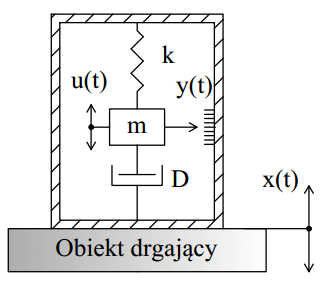
\includegraphics{rys/akcelerometry/wibrometr}
\par\end{centering}

\caption{Model przetwornika sejsmicznego (\emph{�r�d�o:} \cite{Gawedzki2010})
\label{fig:Model-przetwornika-sejsmicznego}}


\end{figure}


Na rysunku \ref{fig:Model-przetwornika-sejsmicznego} pokazano model
przetwornika sejsmicznego. Jego podstawowymi elementami s�:
\begin{itemize}
\item masa sejsmiczna \emph{m},
\item sta�a spr�ysto�ci \emph{k},
\item sta�a t�umienia \emph{D}.
\end{itemize}
Z uwagi na sta�o�� parametr�w \emph{k}, \emph{D} przyjmujemy za�o�enie
co do liniowo�ci przetwornika. Znaczenie wielko�ci \emph{x}, \emph{u},
\emph{y} jest nast�puj�ce:
\begin{itemize}
\item \emph{x(t)} \textendash{} bezwzgl�dne przemieszczenie obudowy przetwornika,
\item \emph{y(t)} \textendash{} przemieszczenie masy sejsmicznej wzgl�dem
obudowy,
\item \emph{u(t)} \textendash{} bezwzgl�dne przemieszczenie masy sejsmicznej.
\end{itemize}
R�wnanie ruchu masy sejsmicznej ma nast�puj�c� posta�:

\begin{equation}
mu''=-ky-Dy'\label{eq:rownanie_ruchu_sejsmiczny_1}
\end{equation}
Ponadto mo�na zauwa�y�, �e:

\begin{equation}
u-x=y\label{eq:zwiazek_miedzy_wspolrzednymi}
\end{equation}
Po przekszta�ceniach otrzymujemy zale�no��:

\begin{equation}
my''+Dy'+ky=-mx''\label{eq:rownanie_ruchu_sejsmiczny_2}
\end{equation}
R�wnanie \ref{eq:rownanie_ruchu_sejsmiczny_2} wi��e bezwzgl�dne przemieszczenie
obudowy z wzgl�dnym przemieszczeniem masy sejsmicznej. Po dokonaniu
podstawie�:

\begin{equation}
\omega_{0}=\sqrt{\frac{k}{m}}\label{eq:pulsacja_drgan_wlasnych}
\end{equation}


\begin{equation}
\xi=\frac{D}{2\sqrt{km}}\label{eq:tlumienie_wzgledne}
\end{equation}
omawiane r�wnanie r�niczkowe mo�e by� zapisane jako:

\begin{equation}
\frac{1}{\omega_{0}^{2}}y''+\frac{2\xi}{\omega_{0}}y'+y=-\frac{1}{\omega_{0}^{2}}x''\label{eq:rownanie_ruchu_sejsmiczny_3}
\end{equation}


W celu wyznaczenia poprawnych warunk�w warunk�w pracy przetwornika,
nale�y pos�u�y� si� analiz� cz�stotliwo�ciow�. W tym celu r�wnanie
\ref{eq:rownanie_ruchu_sejsmiczny_3} poddajemy obustronnie transformacji
Laplace'a (zak�adamy zerowe warunki pocz�tkowe):

\begin{equation}
\frac{1}{\omega_{0}^{2}}s^{2}Y+\frac{2\xi}{\omega_{0}}sY+Y=-\frac{1}{\omega_{0}^{2}}s^{2}X\label{eq:rownanie_ruchu_sejsmiczny_operatorowo}
\end{equation}


gdzie \emph{X} i \emph{Y} s� transformatami sygna��w odpowiednio \emph{x}
i \emph{y}:

\begin{equation}
X\left(s\right)=\mathcal{L}\left\{ x\left(t\right)\right\} \label{eq:laplace_x}
\end{equation}


\begin{equation}
Y\left(s\right)=\mathcal{L}\left\{ y\left(t\right)\right\} \label{eq:laplace_y}
\end{equation}


gdzie $\mathcal{L}\left\{ f\left(t\right)\right\} $oznacza transformacj�
Laplace'a funkcji \emph{f}, okre�lon� wzorem:

\begin{equation}
F\left(s\right)=\mathcal{L}\left\{ f\left(t\right)\right\} =\int_{0}^{+\infty}e^{-st}f\left(t\right)dt\label{eq:laplace_definicja}
\end{equation}


Zmienna \emph{t} jest zmienn�, po kt�rej ca�kujemy i najcz�ciej oznacza
czas, za� \emph{s} jest zmienn� zespolon�, b�d�c� zmienn� niezale�n�
transformaty. Sygna�y poddawane przekszta�ceniu Laplace'a przyj�o
si� nazywa� w literaturze orygina�ami.

Zgodnie z literatur� \cite{Gawedzki2010}, opisywane przetwornik sejsmiczny
mo�e s�u�y� do pomiaru przemieszczenia lub przyspieszenia. Je�eli
za jego transmitancje operatorow� przyjmiemy iloraz transformaty wzgl�dnego
przemieszczenia \emph{Y} oraz transformaty bezwzgl�dnego przyspieszenia
obudowy \emph{s\textsuperscript{\emph{2}}X}, w�wczas taki przetwornik
nazywamy akcelerometrem. Omawiana transmitancja zgodnie ze wzorem
\ref{eq:rownanie_ruchu_sejsmiczny_operatorowo} ma posta�:

\begin{equation}
G\left(s\right)=-\frac{\frac{1}{\omega_{0}^{2}}}{\frac{1}{\omega_{0}^{2}}s^{2}+\frac{2\xi}{\omega_{0}}s+1}\label{eq:transmitancja_akcelerometru_sejsmicznego}
\end{equation}


W celu zbadania w�asno�ci cz�stotliwo�ciowych przetwornika nale�y
pos�u�y� si� transmitancj� widmow�. W tym celu do zale�no�ci \ref{eq:transmitancja_akcelerometru_sejsmicznego}
podstawiamy $s=j\omega$, gdzie \emph{j} jest jednostk� urojon� a
$\omega$ pulsacj�. Otrzymana transmitancja ma posta�:

\begin{equation}
G\left(j\omega\right)=-\frac{\frac{1}{\omega_{0}^{2}}}{-\left(\frac{\omega}{\omega_{0}}\right)^{2}+j2\xi\frac{\omega}{\omega_{0}}+1}\label{eq:transmitancja_widm_akcel_sejsm}
\end{equation}


Wygodniej pos�u�y� si� transmitancj� widmow� w funkcji pulsacji wzgl�dnej:

\begin{equation}
G_{r}\left(j\Omega\right)=-\frac{\frac{1}{\omega_{0}^{2}}}{-\Omega{}^{2}+j2\xi\Omega+1}\label{eq:transmitancja_widm_akcel_sejsm_wzgl}
\end{equation}


gdzie $\Omega=\frac{\omega}{\omega_{0}}$.

Na podstawie zale�no�ci \ref{eq:transmitancja_widm_akcel_sejsm_wzgl}
mo�na wyznaczy� charakterystyki amplitudowe \emph{A} i fazowe $\phi$
akcelerometru \cite{Gawedzki2010}:

\begin{equation}
A\left(j\Omega\right)=\left|G_{r}\left(j\Omega\right)\right|=\frac{1}{\omega_{0}^{2}}\frac{1}{\sqrt{\left(1-\Omega^{2}\right)^{2}+4\xi^{2}\Omega^{2}}}\label{eq:chka_ampl_akcel_sejsm}
\end{equation}


\begin{equation}
\phi\left(j\Omega\right)=arg\left\{ G_{r}\left(j\Omega\right)\right\} =-arctg\left(\frac{2\xi\Omega}{1-\Omega^{2}}\right)\label{eq:chka_fazowa_akcel_sejsm}
\end{equation}


\begin{figure}
\begin{centering}
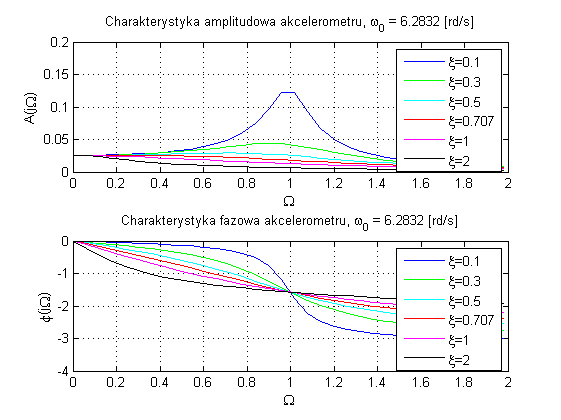
\includegraphics{rys/akcelerometry/chki_akcelerometru}
\par\end{centering}

\caption{Charakterystyki cz�stotliwo�ciowe akcelerometru (\emph{�r�d�o:} \cite{Gawedzki2010})
\label{fig:Charakterystyki-czestotliwosciow}}


\end{figure}


Na rysunku \ref{fig:Charakterystyki-czestotliwosciow} przedstawiono
przebiegi odpowiadaj�ce wzorom \ref{eq:chka_ampl_akcel_sejsm} oraz
\ref{eq:chka_fazowa_akcel_sejsm}. Mo�na zauwa�y�, �e dla dostatecznie
ma�ych t�umie� $\xi$ charakterystyki amplitudowe omawianego akcelerometru
posiadaj� wyra�ne maksimum, dla cz�stotliwo�ci zbli�onych do cz�sto�ci
drga� w�asnych. W przypadku granicznym, gdy t�umienie wynosi zero,
amplituda wzmocnienia d��y do niesko�czono�ci. Omawiane zjawisko nosi
nazw� rezonansu. Aby rezonans m�g� wyst�pi�, musi by� spe�niony warunek
\cite{Gawedzki2010}:

\begin{equation}
\xi<\frac{1}{\sqrt{2}}\thickapprox0.707\label{eq:warunek_rezonansu}
\end{equation}


Maksimum funkcji modu�u transmitancji widmowej jest osi�gane dla pulsacji
wzgl�dnej:

\[
\Omega_{r}=\sqrt{1-2\xi^{2}}
\]


Z literatury \cite{Gawedzki2010} wiadomo, �e warunkiem niezniekszta�caj�cego
przetwarzania sygna�u jest sta�o�� charakterystyki amplitudowej i
liniowo�� charakterystyki fazowej. Bior�c pod uwag� rysunek \ref{fig:Charakterystyki-czestotliwosciow}
mo�na doj�� do wniosku, �e warunki te spe�nione s�, gdy:

\begin{equation}
\omega<\omega_{g}\thickapprox0.5\omega_{0}\label{eq:war_nieznieksztalc_pracy_akcel_sejsm}
\end{equation}


dla t�umienia ograniczonego warunkiem:

\begin{equation}
\xi\in\left(0.6,0.707\right)\label{eq:tlumienie_dla_niezniekszt_pracy_akcel_sejsm}
\end{equation}


W przypadku pulsacji bliskich $\omega_{g}$ nale�y liczy� si� z wi�kszym
b��dem przetwarzania wynikaj�cym ze spadku wzmocnienia i z b��du fazowego
\cite{Gawedzki2010}. Z przebiegu charakterystyk cz�stotliwo�ciowych
wynika, �e pasmo przenoszenia b�dzie tym szersze im wi�ksza b�dzie
pulsacja drga� w�asnych. Mo�na to uzyska� zgodnie z zale�no�ci� \ref{eq:pulsacja_drgan_wlasnych}
poprzez zwi�kszenie sta�ej \emph{k} i zmniejszenie masy sejsmicznej
\emph{m}. Wzrost spr�ysto�ci prowadzi r�wnie� do spadku t�umienia
(zale�no�� \ref{eq:tlumienie_wzgledne}). Pozwala to na uproszczenie
r�wnania (wz�r) do postaci \cite{Gawedzki2010}:

\begin{equation}
y=-\frac{1}{\omega_{0}^{2}}x''=-\frac{1}{\omega_{0}^{2}}a\label{eq:uproszczone_rownanie_ruchu_akcel_sejsm}
\end{equation}


z kt�rej wynika, �e wzgl�dne wychylenie masy przetwornika jest proporcjonalne
do przyspieszenia bezwzgl�dnego. Wsp�czynnik proporcjonalno�ci ��cz�cy
te dwie wielko�ci jest jednak odwrotnie proporcjonalny do kwadratu
pulsacji drga� w�asnych. Wynika z tego, �e ��dania uzyskania szerokiego
pasma przepustowego i du�ej czu�o�ci przetwarzania s� sprzeczne.


\section{Akcelerometr piezorezystancyjny}

\begin{figure}
\begin{centering}
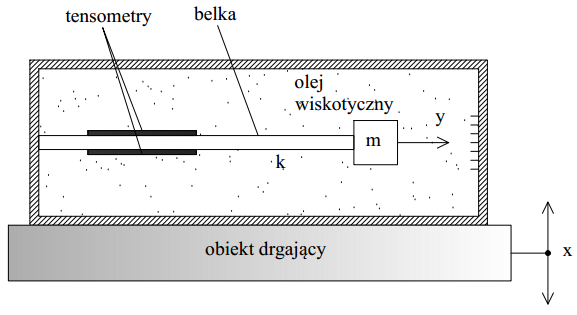
\includegraphics{rys/akcelerometry/piezorezystancyjny}
\par\end{centering}

\caption{Akcelerometr z piezorezystancyjnym czujnikiem tensometrycznym (\emph{�r�d�o:}
\cite{Gawedzki2010}) \label{fig:Akcelerometr-z-piezorezystancyjn}}


\end{figure}


Rysunek \ref{fig:Akcelerometr-z-piezorezystancyjn} przedstawia schemat
akcelerometru z piezorezystancyjnym czujnikiem tensometrycznym. Zasadniczym
elementem przetwornika jest masa sejsmiczna znajduj�ca si� na ko�cu
spr�ystej belki, zamocowanej jednostronnie do obudowy. Drgania masy
na ko�cu belki zachodz� wewn�trz obudowy wype�nionej olejem wiskotycznym.

Mierzone przyspieszenie bezwzgl�dnejest przekszta�cane kolejno na:
\begin{itemize}
\item wzgl�dne przemieszczenie y masy m wzgl�dem obudowy,
\item odkszta�cenie $\varepsilon$ wzgl�dne belki,
\item wzgl�dn� zmian� rezystancji $\varepsilon_{R}$ czujnika tensometrycznego,
\item wzgl�dn� zmian� napi�cia nier�wnowagi $\frac{\Delta U}{U_{Z}}$ mostka
($\Delta U$ oznacza przyrost napi�cia niezr�wnowa�enia mostka, za�
\emph{U\textsubscript{\emph{Z}}} napi�cie zasilaj�ce mostek).
\end{itemize}
Poniewa� cz�stotliwo�� drga� w�asnych tego typu przetwornik�w s� stosunkowo
niskie (od kilkuset herc�w do kilku kiloherc�w), niewielkie jest r�wnie�
ich pasmo przenoszenia. Do zalet tego typu konstrukcji mo�na zaliczy�
mo�liwo�� pomiaru sta�ych przyspiesze� \cite{Gawedzki2010}. Czu�o��
przetwornika mo�na wyznaczy� z nast�puj�cej zale�no�ci \cite{Gawedzki2010}:

\begin{equation}
S_{a}=\frac{\frac{\Delta U_{-g}^{g}}{U_{Z}}}{2g}\label{eq:czulosc_akcel_piezorez}
\end{equation}


gdzie $\Delta U_{-g}^{g}$ oznacza przyrost napi�cia nier�wnowagi
mostka przy zmianie pomiaru przyspieszenia z \emph{g} na \emph{-g}.

Uk�ady podobne do powy�szego s� wytwarzane w technice mikromaszynowej
MEMS, pozwalaj�cej na znaczne zmniejszenie rozmiaru przetwornika.
W akcelerometrach takich do przetwarzania zmiany odkszta�cenia na
zmian� rezystancji wykorzystuje si� tensometry piezorezystywne.

Wspomniana technika MEMS pozwala r�wnie� na produkcj� przyspieszeniomierzy
pojemno�ciowych, stosowanych bardzo cz�sto jako elementy uk�ad�w bezpiecze�stwa
czynnego w samochodach (wyzwalacze poduszek powietrznych). Przyk�ad
konstrukcji takiego akcelerometru pokazano na rysunku \ref{fig:mems-pojemnosciowy}.

\begin{figure}
\begin{centering}
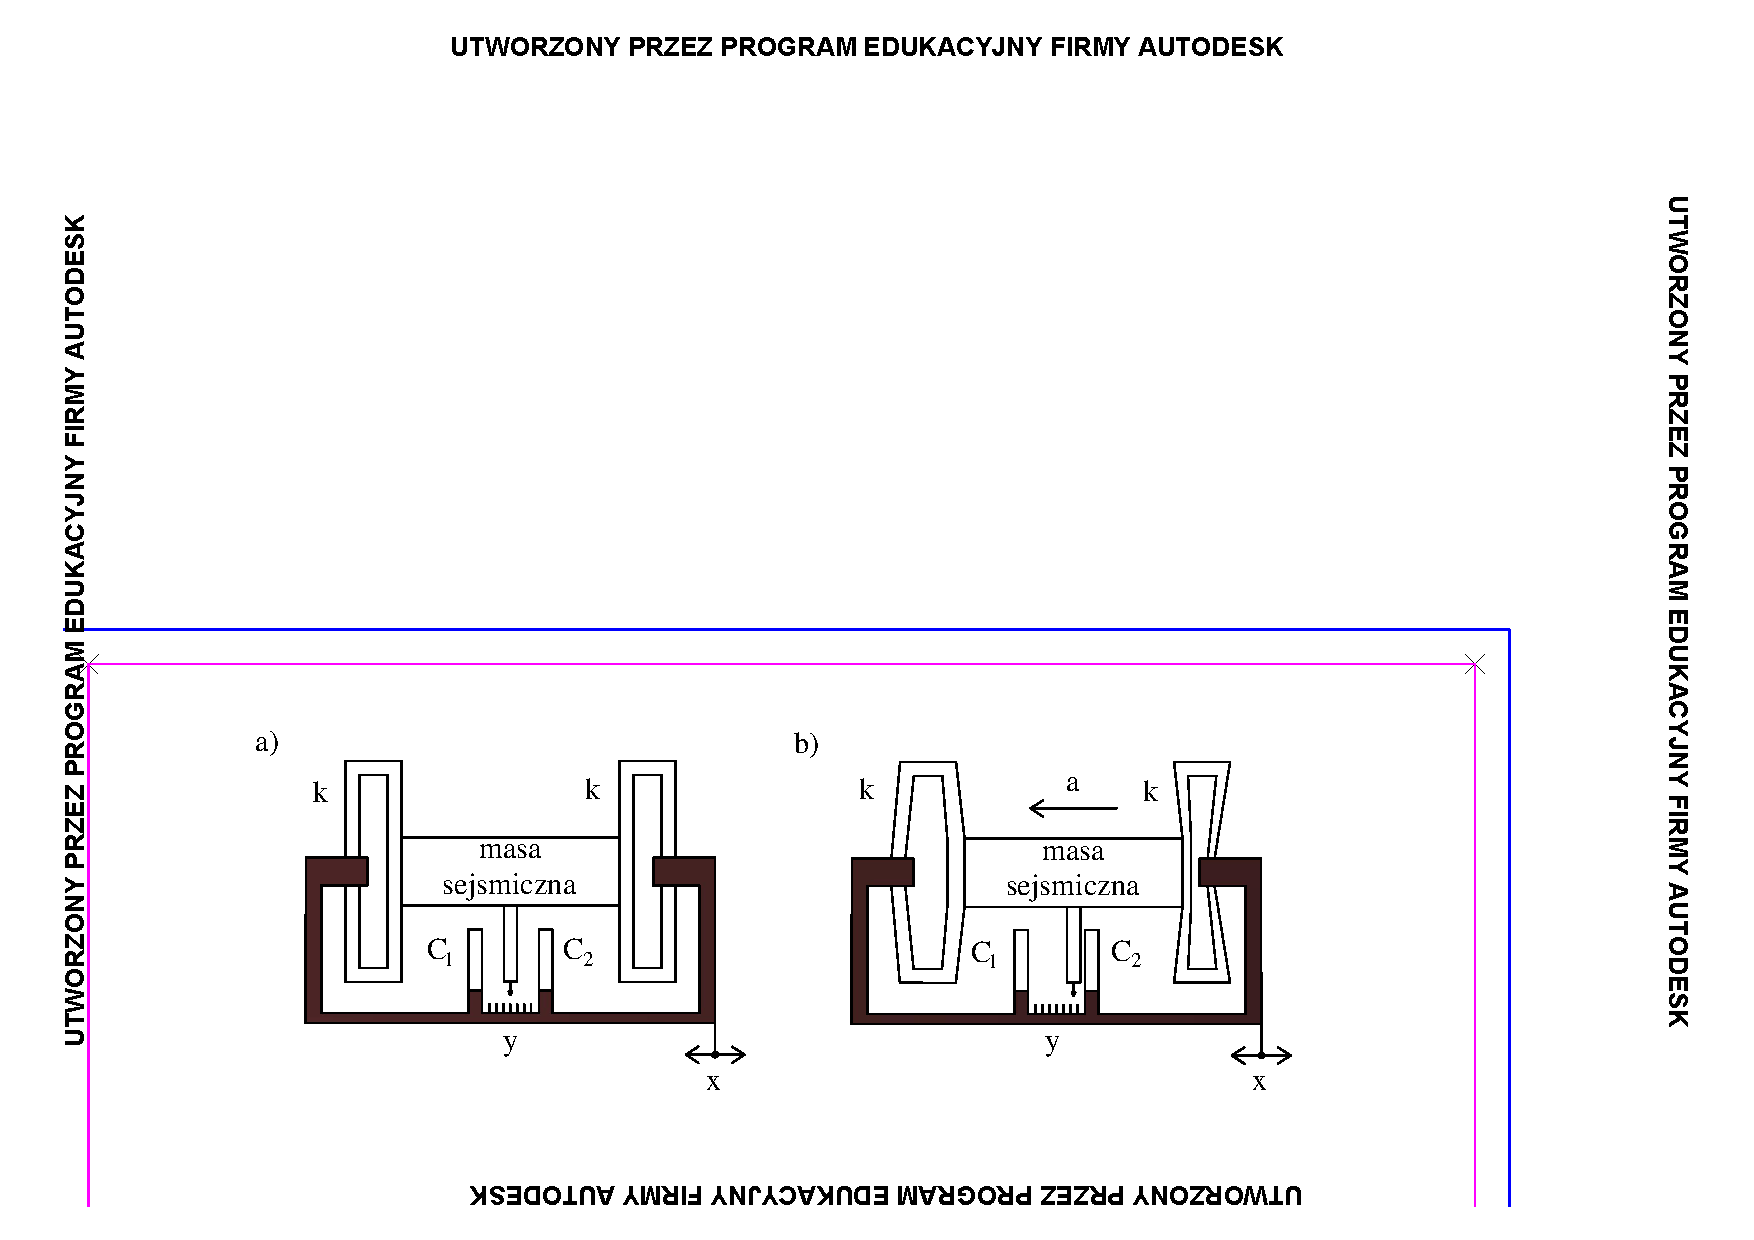
\includegraphics{rys/akcelerometry/mems}
\par\end{centering}

\caption{Zasada dzia�ania akcelerometru pojemno�ciowego: a) uk�ad znajduj�cy
si� w spoczynku, b) uk�ad poddawany dzia�aniu przyspieszenia \textbf{\emph{a}}\emph{
}(\emph{�r�d�o:} \cite{Gawedzki2010}) \label{fig:mems-pojemnosciowy}}


\end{figure}


Podstawowym elementem przetwornika jest p�yta, stanowi�ca mas� sejsmiczn�,
kt�rej ko�ce zamocowane s� poprzez spr�yste uchwyty do obudowy. Z
p�yt� po��czona jest elektroda, znajduj�ca si� pomi�dzy dwiema innymi,
ale nieruchomymi (wzgl�dem obudowy) elektrodami, po��czonymi z obudow�.
Ca�o�� tworzy r�nicowy uk�ad dw�ch kondensator�w \emph{C\textsubscript{\emph{1}}}
i \emph{C\textsubscript{\emph{2}}}, kt�rych pojemno�ci zale�� od
po�o�enia �rodkowej ok�adki, kt�re z kolei zale�y od wychylenia masy
sejsmicznej. Do ok�adek nieruchomych przyk�ada si� prostok�tne napi�cia
znajduj�ce si� w przeciwfazie.

Je�eli uk�ad nie jest poddawany dzia�aniu przyspieszenia, pojemno�ci
\emph{C\textsubscript{\emph{1}}} i \emph{C\textsubscript{\emph{2}}}
s� r�wne, a napi�ciowy sygna� wyj�ciowy ze �rodkowej elektrody ma
warto�� zerow�. Dzia�anie przyspieszenia powoduje wychylenie masy
sejsmicznej oraz �rodkowej ok�adki, co prowadzi do zmniejszenia jednej
z pojemno�ci i zwi�kszenia drugiej. Niezerowy ju� sygna� z ruchomej
elektrody jest demodulowany i przetwarzany przez wzmacniacz buforowy
\cite{Gawedzki2010}. Ca�y uk�ad pomiarowy posiada p�tl� ujemnego
sprz�enia zwrotnego, utrzymuj�cego �rodkow� elektrod� w po�o�eniu
r�wnowagi. Miar� przyspieszenia jest warto�� napi�cia wyj�ciowego
akcelerometru, niezb�dna do utrzymania �rodkowej ok�adki w po�o�eniu
r�wnowagi \cite{Gawedzki2010}.


\section{Przetworniki piezoelektryczne}


\subsection{Zasada dzia�ania}

Dzia�anie tego typu przetwornik�w polega na wykorzystaniu zjawiska
piezoelektrycznego. Polega ono na pojawianiu si� �adunku elektrycznego
na powierzchni �adunku pod wp�ywem istniej�cych napr�e� mechanicznych.
Kryszta�y, kt�re cechuj� si� omawianymi w�asno�ciami nazywane s� piezoelektrykami.
W naturze istnieje r�wnie� zjawisko odwrotne (nazywane zjawiskiem
piezoelektrycznym odwrotnym, w odr�nieniu od prostego), polegaj�ce
na zmianie wymiar�w kryszta�u pod wp�ywem przy�o�onego pola elektrycznego. 

W praktyce jako piezoelektryka najcz�ciej u�ywa si� krzemu (SiO\textsubscript{2}).
Do jego zalet mo�na zaliczy� stosunkowo du�� wytrzyma�o�� mechaniczn�,
znaczn� rezystywno�� i sta�� piezoelektryczn� i niewielk� zale�no��
zjawiska piezoelektrycznego od temperatury.

Na rysunku przedstawiono schematycznie budow� kryszta�u kwarcu. Jak
wida� jego kom�rka elementarna ma posta� uk�adu heksagonalnego. Przy�o�enie
do p�ytki kwarcowej si�y powoduje przemieszczenie si� jon�w krzemu
i tlenu, co skutkuje pojawieniem si� �adunk�w na jej powierzchni oraz
pola elektrycznego w jej wn�trzu. Kierunek pola zale�y od kierunku
dzia�ania si�y oraz od sposobu wyci�cia p�ytki wzgl�dem osi krystalograficznych
kwarcu, za� jego warto�� od warto�ci dzia�aj�cej si�y.

\begin{figure}
\begin{centering}
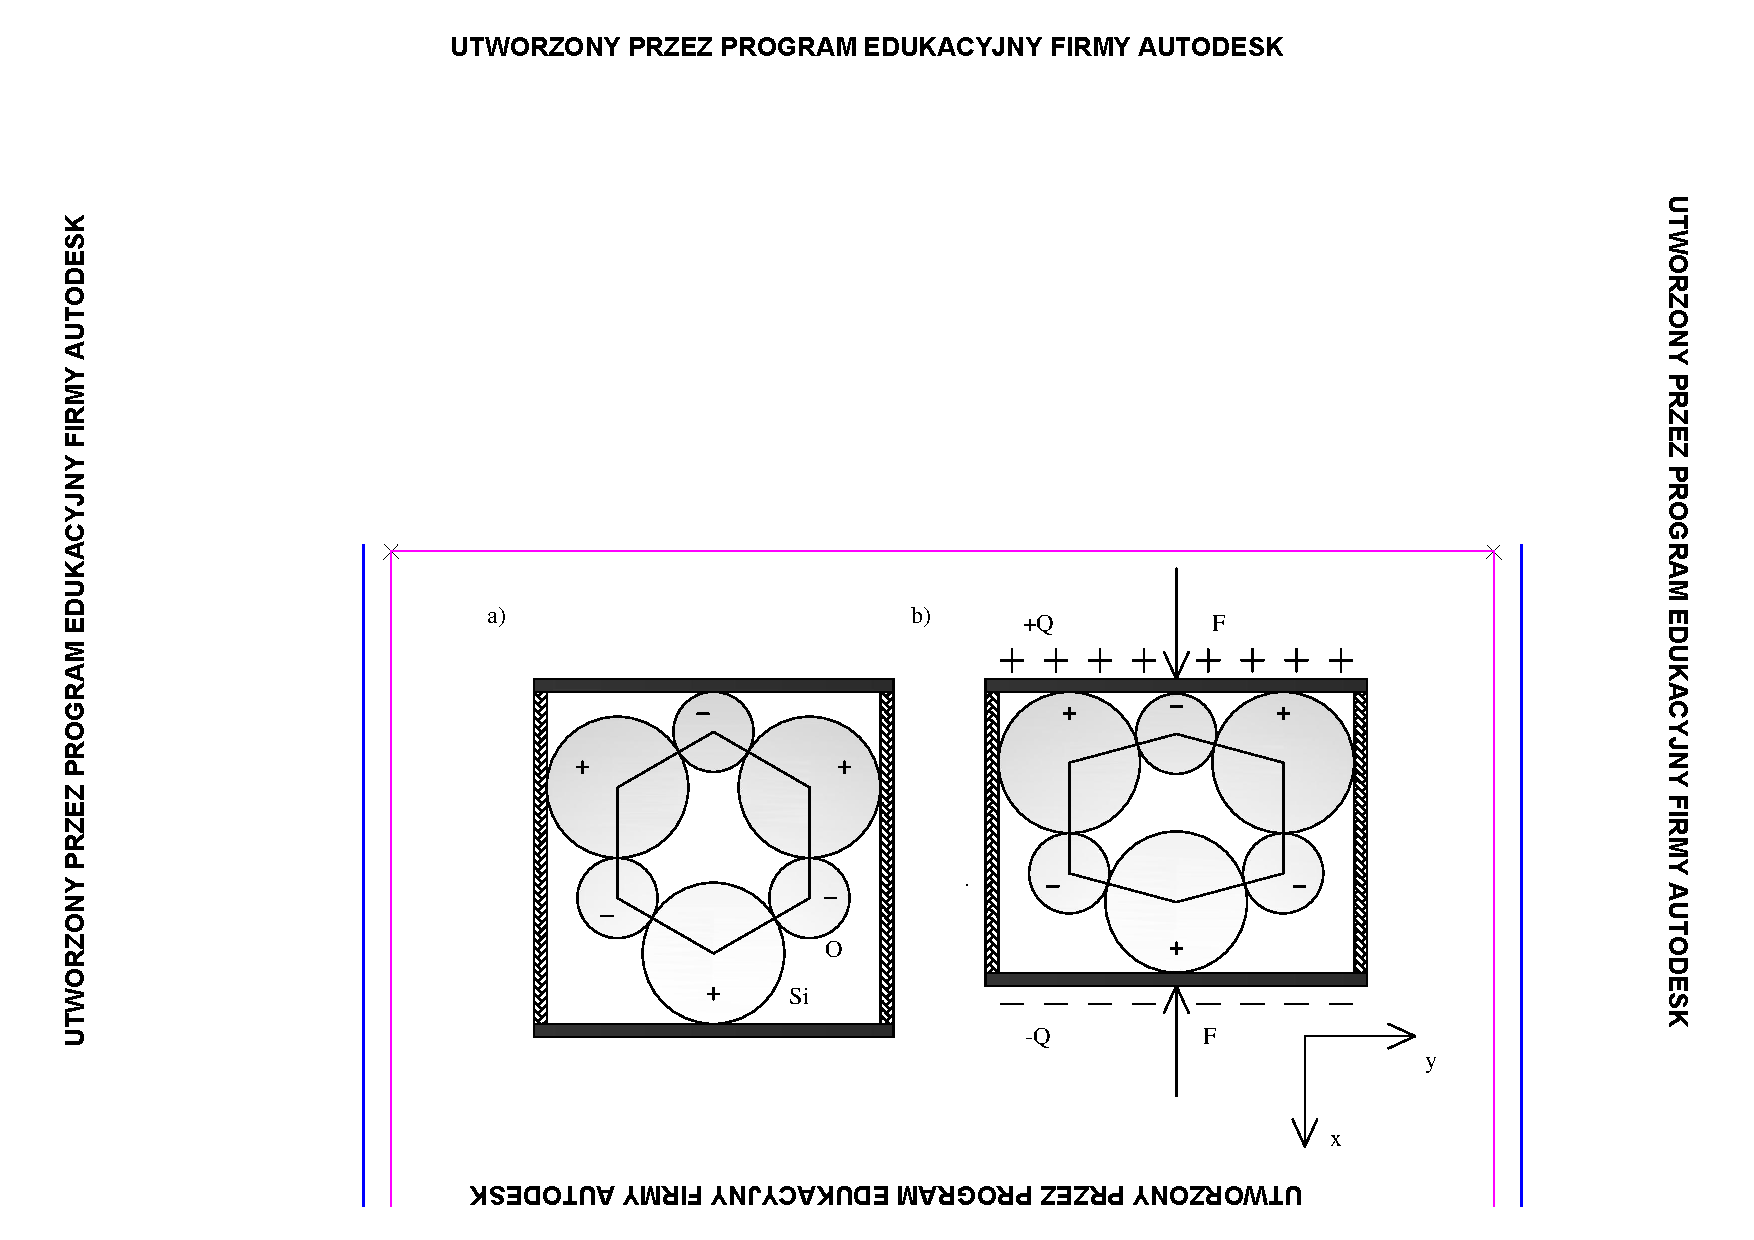
\includegraphics{rys/akcelerometry/kwarc}
\par\end{centering}

\caption{Ilustracja efektu piezoelektrycznego wzd�u�nego na przyk�adzie kryszta�u
kwarcu: a) kryszta� nieobci��ony, b) kryszta� poddany dzia�aniu si�y
\textbf{\emph{F}} (\emph{�r�d�o:} \cite{Gawedzki2010}) \label{fig:Ilustracja-efektu-piezoelektrycz}}


\end{figure}


Do osi krystalicznych kwarcu mo�na zaliczy� \cite{Gawedzki2010}:
\begin{itemize}
\item trzy osie elektryczne, ��cz�ce przeciwleg�e wierzcho�ki sze�ciok�ta,
\item trzy osie mechaniczne, ��cz�ce �rodki przeciwleg�ych bok�w sze�ciok�ta,
\item o� optyczn�, prostopad�� do p�aszczyzny sze�ciok�ta.
\end{itemize}
Je�li si�a \emph{F} dzia�a wzd�u� osi \emph{x}, to �adunki generowane
s� na powierzchniach do niej prostopad�ych. Odkszta�canie kryszta�u
wzd�u� osi \emph{y} powoduje powstawanie �adunk�w r�wnie� na tych
samych powierzchniach. W pierwszym przypadku mamy do czynienia ze
zjawiskiem piezoelektrycznym wzd�u�nym, za� w drugim z poprzecznym.

W przypadku zjawiska wzd�u�nego, g�sto�� \emph{q} �adunku wygenerowanego
na powierzchni \emph{A\textsubscript{\emph{x}}} prostopad�ej do osi
elektrycznej \emph{x}, wzd�u� kt�rej dzia�a si�a \emph{F} wynosi \cite{Gawedzki2010}:

\begin{equation}
q=k_{p}\sigma\label{eq:gestosc_ladunku_piezoelektryk}
\end{equation}


gdzie:
\begin{itemize}
\item \emph{k\textsubscript{\emph{p}}} \textendash{} sta�a (tzw. modu�
piezoelektryczny),
\item $\sigma$ - napr�enie powsta�e w p�ytce, w wyniku dzia�ania si�y
\emph{F}.
\end{itemize}
Napr�enie wyst�puj�ce w ostatnim wzorze mo�e by� wyznaczone w nast�puj�cy
spos�b:

\begin{equation}
\sigma=\frac{F}{A_{x}}\label{eq:naprezenie}
\end{equation}


Warto�� �adunku \emph{Q} zgromadzonego na powierzchni krzemu wyniesie
zatem:

\begin{equation}
Q=qA_{x}=k_{p}F\label{eq:ladunek_piezoelektryk}
\end{equation}


a napi�cie \emph{U} mi�dzy powierzchniami p�ytki b�dzie mia�o warto��:

\begin{equation}
U=\frac{Q}{C}\label{eq:napiecie_piezoelektryk}
\end{equation}


gdzie \emph{C} jest sum� pojemno�ci p�ytki i obwodu pomiarowego \cite{Gawedzki2010}.
Czu�o�� �adunkowa wynosi:

\begin{equation}
S_{Q}=\frac{dQ}{dF}=k_{p}\label{eq:czulosc_ladunkowa_piezoelektryka}
\end{equation}


za� napi�ciowa:

\begin{equation}
S_{U}=\frac{dU}{dF}=\frac{1}{C}S_{Q}=\frac{k_{p}}{C}\label{eq:czulosc_napieciowa_piezoelektryka}
\end{equation}


Jak wida� z powy�szych wzor�w, czu�o�� �adunkowa piezoelektryka jest
wielko�ci� sta��, za� czu�o�� napi�ciowa zale�y od pojemno�ci przewod�w
i wzmacniacza pomiarowego.


\subsection{W�asno�ci dynamiczne}

\begin{figure}
\begin{centering}
\includegraphics{rys/akcelerometry/piezo_zastepczy}
\par\end{centering}

\caption{W�asno�ci toru pomiarowego z przetwornikiem piezoelektrycznym w zakresie
niskich cz�stotliwo�ci: a) model toru, b) schemat zast�pczy (\emph{�r�d�o:}
\cite{Gawedzki2010}) \label{fig:schemat-toru-pomiarowego}}


\end{figure}


P�ytka piezoelektryka posiada cz�stotliwo�� rezonansow� drga� zale�n�
od jej masy \emph{m}, i spr�ysto�ci \emph{k}. Je�li uwzgl�dnimy,
�e p�ytka taka jest obiektem o parametrach roz�o�onych, a nie skupionych
(jak w omawianym poprzednio modelu), to nale�y pami�ta�, �e b�dzie
ona mog�a posiada� kilka cz�stotliwo�ci rezonansowych. Najni�sza z
nich ogranicza pasmo przetwarzania przetwornika od g�ry. W celu okre�lenia
dolnego ograniczenia, mo�na pos�u�y� si� modelem toru pomiarowego
ukazanego na rysunku \ref{fig:schemat-toru-pomiarowego}, wykorzystuj�cego
przetwornik piezoelektryczny. Tor sk�ada si� z nast�puj�cych element�w:
\begin{itemize}
\item p�ytki piezoelektrycznej o rezystancji \emph{R\textsubscript{\emph{c}}}
i pojemno�ci \emph{C\textsubscript{\emph{c}}},
\item przewod�w ��czeniowych o rezystancji \emph{R\textsubscript{\emph{k}}}
i pojemno�ci \emph{C\textsubscript{\emph{k}}},
\item wzmacniacza pomiarowego o rezystancji wej�ciowej \emph{R\textsubscript{\emph{o}}}
i pojemno�ci wej�ciowej \emph{C\textsubscript{\emph{o}}},
\item przetwornika piezoelektrycznego pe�ni�cego rol� generatora �adunku.
\end{itemize}
Dla obwod�w z rysunku \ref{fig:schemat-toru-pomiarowego} mo�na napisa�
nast�puj�ce zale�no�ci:

\begin{equation}
C=C_{c}+C_{k}+C_{o}\label{eq:pojemnosc_zastepcza_toru}
\end{equation}


\begin{equation}
\frac{1}{R}=\frac{1}{R_{c}}+\frac{1}{R_{k}}+\frac{1}{R_{o}}\label{eq:rezystancja_zastepcza_toru}
\end{equation}


\begin{equation}
i=i_{C}+i_{R}\label{eq:prad_wypadkowy_w_torze}
\end{equation}


\begin{equation}
\frac{dQ}{dt}=C\frac{du}{dt}+\frac{u}{R}\label{eq:rownanie_pradow_w_torze}
\end{equation}


Ostatnie r�wnanie mo�na zapisa� w postaci operatorowej (zak�adamy
zerowe warunki pocz�tkowe):

\begin{equation}
sQ\left(s\right)=sCU\left(s\right)+\frac{1}{R}U\left(s\right)\label{eq:rownanie_pradow_operatorowo}
\end{equation}


Traktuj�c \emph{Q(t)} jako sygna� wej�ciowy, za� napi�cie \emph{u(t)}
jako sygna� wyj�ciowy, mo�emy wyznaczy� transmitancj� \emph{K\textsubscript{\emph{p}}(s)}
operatorow� toru:

\begin{equation}
K_{p}\left(s\right)=\frac{Rs}{RCs+1}\label{eq:transmitancja_toru}
\end{equation}


Transmitancja widmowa ma posta�:

\begin{equation}
K_{p}\left(j\omega\right)=\frac{jR\omega}{jRC\omega+1}\label{eq:transmitancja_widmowa_toru}
\end{equation}


Na tej podstawie wyznaczamy charakterystyk� amplitudow�:

\begin{equation}
\left|K_{p}\left(j\omega\right)\right|=\frac{R\omega}{\sqrt{1+\left(RC\omega\right)^{2}}}\label{eq:chka_amplitudowa_toru}
\end{equation}


oraz fazow�:

\begin{equation}
\phi\left(\omega\right)=arg\left\{ K_{p}\left(j\omega\right)\right\} =arg\left\{ \frac{jR\omega}{jRC\omega+1}\right\} \label{eq:chka_fazowa_toru}
\end{equation}


\begin{figure}
\begin{centering}
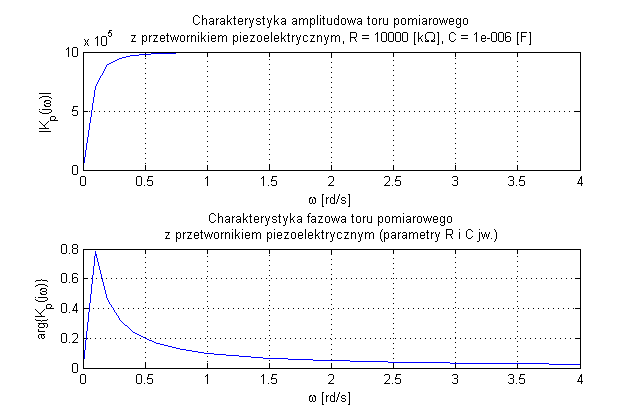
\includegraphics{rys/akcelerometry/piezoel_charakterystyki}
\par\end{centering}

\caption{Charakterystyki cz�stotliwo�ciowe toru pomiarowego z przetwornikiem
piezoelektrycznym \label{fig:Charakterystyki-amplitudowe-toru}}


\end{figure}


Obie charakterystyki pokazano na rysunku \ref{fig:Charakterystyki-amplitudowe-toru}.
Jak wida� uk�ad nie przenosi niskich cz�stotliwo�ci. W szczeg�lno�ci
nie jest mo�liwy pomiar sygna��w sta�ych. Wynika to z tego, �e gromadzony
na powierzchni piezoelektryka �adunek, roz�adowuje si� przez sko�czon�
rezystancj� toru pomiarowego. Dolna pulsacja graniczna toru wynosi
\cite{Gawedzki2010}:

\begin{equation}
\omega_{d}=\frac{1}{RC}\label{eq:dolna_pulsacja_gr_toru}
\end{equation}


i ro�nie ze wzrostem rezystancji \emph{R} i pojemno�ci \emph{C}. Aby
poszerzy� pasmo przenoszenia, omawiana cz�sto�� musi by� jak najmniejsza.
Zwi�kszanie pojemno�ci uk�adu jest niekorzystne ze wzgl�du na spadek
czu�o�ci napi�ciowej \ref{eq:czulosc_napieciowa_piezoelektryka} oraz
warto�ci napi�cia \ref{eq:napiecie_piezoelektryk}. Nale�y wi�c zapewni�
jak najwi�ksz� warto�� rezystancji zast�pczej \emph{R}, co nak�ada
du�e wymagania jako�ciowe na wzmacniacz pomiarowy oraz przewody ��cz�ce
go z czujnikiem piezoelektrycznym. Zwykle rezystancja kwarcowego przetwornika
piezoelektrycznego osi�ga warto�ci rz�du 10\textsuperscript{15}$\Omega$
\cite{Gawedzki2010}.


\subsection{Akcelerometr piezoelektryczny}

\begin{figure}
\begin{centering}
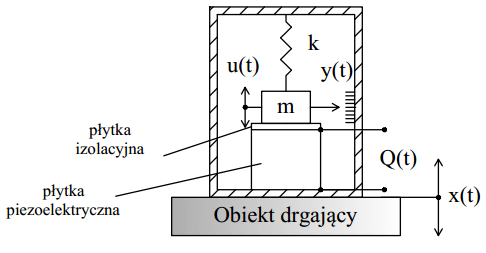
\includegraphics{rys/akcelerometry/piezoelektryczny}
\par\end{centering}

\caption{Model akcelerometru piezoelektrycznego (\emph{�r�d�o:} \cite{Gawedzki2010})
\label{fig:Model-akcelerometru-piezoelektry}}


\end{figure}


Zasada dzia�ania akcelerometru piezoelektrycznego polega na wytwarzaniu
�adunku elektrycznego na powierzchni piezoelektryka, w wyniku oddzia�ywania
masy sejsmicznej poddawanej dzia�aniu si�y bezw�adno�ci. Warto�� �adunku
zale�y od warto�ci si�y, za� znak od tego czy kryszta� jest �ciskany
czy rozci�gany.

Na rysunku \ref{fig:Model-akcelerometru-piezoelektry} pokazano model
akcelerometru piezoelektrycznego. Oddzia�ywanie z p�ytk� piezoelektryka
zachodzi wzd�u� jego osi elektrycznej, za� �adunek generowany jest
na powierzchniach prostopad�ych do niej. Spr�yna wywiera wst�pny
nacisk masy, kt�rego warto�� zmienia si� w zale�no�ci od mierzonego
przyspieszenia.

Si�� bezw�adno�ci, z jak� masa sejsmiczna dzia�a na przetwornik, mo�e
by� wyznaczona z zale�no�ci:

\begin{equation}
F_{b}=mu''\label{eq:sila_bezwladnosci}
\end{equation}


Uwzgl�dniaj�c zale�no�� \ref{eq:ladunek_piezoelektryk} ��cz�c� si��
z �adunkiem, mo�na napisa� �e:

\begin{equation}
mu''=\frac{1}{k_{p}}Q\label{eq:sila_bezwl_ladunek}
\end{equation}


Przy za�o�eniu zerowych warunk�w pocz�tkowych, transformata napi�cia
\emph{u(t)} ma posta�:

\begin{equation}
U\left(s\right)=\frac{1}{k_{p}ms^{2}}Q\left(s\right)\label{eq:napiecie_ladunek_operatorowo}
\end{equation}


R�wnanie ruchu masy mo�na zapisa� jako:

\begin{equation}
mu''+cy'+ky=0\label{eq:rownanie_ruchu_piezo_1}
\end{equation}


co po uwzgl�dnieniu zale�no�ci mi�dzy przemieszczeniami prowadzi do
zwi�zku:

\begin{equation}
mu''+cu'+ku=cx'+kx\label{eq:rownanie_ruchu_piezo_2}
\end{equation}


Maj�c na uwadze podstawienia \ref{eq:pulsacja_drgan_wlasnych} i \ref{eq:tlumienie_wzgledne},
mo�na powy�sz� zale�no�� zapisa� operatorowo w nast�puj�cy spos�b:

\begin{equation}
\frac{1}{\omega_{0}^{2}}s^{2}U\left(s\right)+\frac{2\xi}{\omega_{0}}sU\left(s\right)=\frac{2\xi}{\omega_{0}}sX\left(s\right)+X\left(s\right)\label{eq:rownanie_ruchu_piezo_operatorowo}
\end{equation}


Transmitancja operatorowa, wi���ca bezwzgl�dne przemieszczenie masy
\emph{u} z bezwzgl�dnym przemieszczeniem \emph{x} obiektu ma posta�:

\begin{equation}
G_{U}\left(s\right)=\frac{U\left(s\right)}{X\left(s\right)}=\frac{\frac{2\xi}{\omega_{0}}s+1}{\frac{1}{\omega_{0}^{2}}s^{2}+\frac{2\xi}{\omega_{0}}s+1}\label{eq:transmitancja_napieciowa_piezo}
\end{equation}


Je�li za sygna� wyj�ciowy przyjmiemy nie napi�cie lecz �adunek, w�wczas
transmitancja przyjmie posta�:

\begin{equation}
G_{Q}\left(s\right)=mk_{p}s^{2}\frac{\frac{2\xi}{\omega_{0}}s+1}{\frac{1}{\omega_{0}^{2}}s^{2}+\frac{2\xi}{\omega_{0}}s+1}\label{eq:transmitancja_ladunkowa_piezo}
\end{equation}


Poniewa� w akcelerometrach piezoelektrycznych pulsacja drga� w�asnych
ma du�� warto�� (ma�a masa sejsmiczna i du�a sztywno�� spr�yny) a
t�umienie niewielk� (ok. 0.01) \cite{Gawedzki2010}, wi�c ostatnie
r�wnanie mo�e by� zapisane w prostszy spos�b:

\begin{equation}
G_{Q}\left(s\right)=mk_{p}s^{2}\label{eq:transmitancja_ladunkowa_piezo_uproszczona}
\end{equation}


z czego wynika, �e w dziedzinie czasu zachodzi relacja:

\begin{equation}
Q=mk_{p}x''\label{eq:uproszczone_rown_ruchu_piezo}
\end{equation}


a zatem generowany �adunek jest proporcjonalny do przyspieszenia drgaj�cego
obiektu.



\chapter{�yroskopy i ich zastosowanie w elektronice u�ytkowej}


\section{Budowa i zasada dzia�ania}

�yroskop jest urz�dzeniem s�u��cym do pomiaru lub utrzymywania po�o�enia
k�towego. Dzia�a w oparciu o zasad� zachowania momentu p�du. Zwykle
jego zasadniczym elementem jest ruchomy kr��ek, kt�ry wprawiony w
szybki ruch obrotowy zachowuje po�o�enie swojej osi obrotu, z niewielkimi
ruchami precesyjnymi, kt�re mog� zosta� wyeliminowane dzi�ki zastosowaniu
t�umienia. Aby poprawna praca �yroskopu by�a mo�liwa, konieczne jest
zapewnienie szybkiej pr�dko�ci obrotowej kr��ka oraz dobrych warunk�w
�o�yskowania. Wymagaj� one zminimalizowania tarcia, co mo�na osi�gn��
poprzez poprzez �o�yskowanie na strumieniu powietrza, lub zawieszeniu
w polu elektrostatycznym (lub magnetycznym) w pr�ni. Przedmiotem
znanym z �ycia codziennego, kt�ry wprawiony w szybki ruch obrotowy
zachowuje si� jak �yroskop jest b�k.
\begin{figure}
\begin{centering}
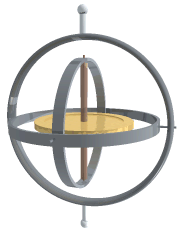
\includegraphics{rys/zyroskopy/zyroskop}
\par\end{centering}

\caption{Jedna z mo�liwych konstrukcji �yroskopu (\emph{�r�d�o:} \cite{zyro_wiki})\label{fig:zyroskop}}


\end{figure}


Na rysunku \ref{fig:zyroskop} pokazano przyk�adow� konstrukcj� �yroskopu.
W jego centralnym miejscu znajduje si� kr��ek zawieszony na podw�jnej
ramce. Je�li nadamy mu du�� pr�dko�� obrotow�, to zachowa on po�o�enie
osi obrotu, cho� mo�liwe b�dzie wyst�pienie ruch�w precesyjnych.

Dla ruchu obrotowego prawdziwa jest zale�no��:

\begin{equation}
\overrightarrow{M}=I\overrightarrow{\varepsilon}\label{eq:kret-II-zasada}
\end{equation}


gdzie:
\begin{itemize}
\item $\overrightarrow{M}$ - wektor momentu si�y przy�o�onego do bry�y,
\item \emph{I} - moment bezw�adno�ci bry�y sztywnej,
\item $\overrightarrow{\varepsilon}$ - wektor przyspieszenia k�towego (bry�y).
\end{itemize}
Moment si�y powoduje zmian� momentu p�du:

\begin{equation}
\overrightarrow{M}=\frac{d\overrightarrow{L}}{dt}\label{eq:moment-sily-moment-pedu}
\end{equation}


gdzie $\overrightarrow{L}$ jest wektorem momentu p�du.

\begin{figure}
\begin{centering}
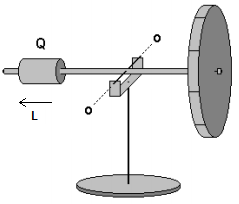
\includegraphics{rys/zyroskopy/zyroskop2}
\par\end{centering}

\caption{Inna konstrukcja �yroskopu (\emph{�r�d�o: }\cite{zyro_am_gdynia})
\label{fig:zyroskop2}}


\end{figure}


Wielko�� $\overrightarrow{L}$ wyznacza si� z nast�puj�cego wzoru:

\begin{equation}
\overrightarrow{L}=I\overrightarrow{\omega}\label{eq:moment_pedu}
\end{equation}


gdzie $\overrightarrow{\omega}$ jest pr�dko�ci� k�tow� bry�y sztywnej.

Zjawisko precesji wyst�puj�ce w �yroskopach mo�na opisa� na przyk�adzie
konstrukcji z rysunku \ref{fig:zyroskop2}. Je�eli ci�ar moment si�y
poch�dz�cy od ci�aru \emph{Q} r�wnowa�y moment si�y pochodz�cy od
ci�aru kr��ka, w�wczas �yroskop wykouje ruch obrotowy wok� swojej
osi (prostej prostopad�ej do p�aszczyzny kr��ka i przechodz�cej przez
jego �rodek). Je�li zwi�kszymy ci�ar \emph{Q} (lub przesuniemy ci�arek
w lewo lub prawo), pojawi si� dodatkowy moment si�y dzia�aj�cy prostopadle
do $\overrightarrow{L}$. Spowoduje on, �e dotychczasowa o� obrotu
kr��ka zacznie si� obraca� wok� dotychczasowego po�o�enia, zakre�laj�c
przy tym powierzchni� boczn� sto�ka. Ruch ten nazywa si� precesyjnym,
za� cz�sto�� precesji jest wprost proporcjonalna do momentu, kt�ry
j� wywo�uje i odwrotnie proporcjonalna do momentu bezw�adno�ci i cz�sto�ci
ruchu obrotowego kr��ka:

\begin{equation}
f_{p}=\frac{M_{p}}{4\pi^{2}If_{r}}\label{eq:czest-precesji}
\end{equation}


gdzie:
\begin{itemize}
\item $f_{p}$ - cz�stotliwo�� precesji,
\item $M_{p}$ - moment si�y powoduj�cy wyst�pienie precesji (prostopad�y
do pierwotnego momentu p�du $\overrightarrow{L}$),
\item \emph{I} - moment bezw�adno�ci,
\item $f_{r}$ - cz�sto�� ruchu oobrotowego kr��ka.
\end{itemize}
Opisane zjawisko okre�la si� mianem precesji wymuszonej, gdy� wywo�ana
jest przez moment $\overrightarrow{M_{p}}$. Pr�cz tego mo�liwa jest
tak�e precesja swobodna, wyst�puj�ca gdy o� wok� kt�rej obraca si�
swobodnie bry�a, nie pokrywa si� z �adn� z osi g��wnych tensora momentu
bezw�adno�ci tej bry�y.


\section{Podzia� �yroskop�w}

�yroskopy mo�na podzieli� na dwie grupy - kierunkowe oraz pr�dko�ciowe.
W przypadku tych pierwszych, zasadniczym elementem jest szybko wiruj�cy
obiekt, maj�cy zwykle posta� dysku, zawieszony w konstrukcji pozwalaj�cej
na swobodny obr�t wok� uk�adu odniesienia (np. cia�a do kt�rego umocowany
jest �yroskop). Mo�na to uzyska� dzi�ki zastosowaniu odpowiednich
przegub�w o osi obrotu prostopad�ej do osi obrotu wiruj�cej bry�y.
Takie rozwi�zanie zmniejsza wp�yw obrot�w cia�a na �yroskop, kt�ry
d��y do zachowania sta�ego po�o�enia.

Przeznaczeniem �yroskop�w pr�dko�ciowych jest wskazywanie pr�dko�ci
k�towej obiektu, na kt�rym s� umiejscowione. Zaliczamy do nich konstrukcje
mechaniczne (kt�rych wad� jest ograniczona swoboda w ruchu obrotowym)
a tak�e �yroskopy optyczne (laserowe i �wiat�owodowe) oraz konstrukcje
wykorzystuj�ce zjawisko Coriolisa.


\section{�yroskopy w elektronice u�ytkowej}

\begin{figure}
\begin{centering}
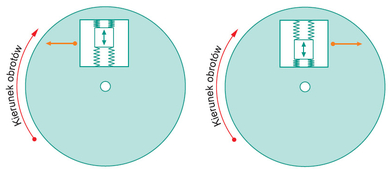
\includegraphics{rys/zyroskopy/zyroskop_coriolis}
\par\end{centering}

\caption{�yroskop MEMS (\emph{�r�d�o: }\cite{elektronikab2b}) \label{fig:zyroskop-MEMS}}


\end{figure}


�yroskopy s� elementem wielu urz�dze� elektrycznych, w kt�rych nale�y
mierzy� lub rejestrowa� zmiany po�o�enia (np. wska�niki komputerowe,
myszki, smartfony). Mog� by� one wytwarzane w technologii MEMS (o
ktorej wspomniano w rozdziale o akcelerometrach), przy czym dotyczy
to g��wnie �yroskop�w pr�dko�ciowych. Konstrukcje takie wykorzystuj�
efekt Coriolisa, a ich pogl�dowy schemat pokazano na rysunku \ref{fig:zyroskop-MEMS}.
Zasadniczym elementem jest masa, wytrawiana w polikrzemie i przytwierdzona
do krzemowej ramy tak, aby mog�a wykonywa� ruchy tylko w jednym kierunku.
Maj� one posta� drga� mo�liwych, dzi�ki zawieszeniu masy na spr�ynach.
Ca�o�� jest umieszczona na platformie wykonuj�cej ruch obrotowy. Gdy
masa porusza si� w kierunku brzegu tarczy, dzia�a na ni� si�a skierowana
w prawo. Jednocze�nie sama masa oddzia�uje na ram� si�� skierowana
w lewo. W trakcie przemieszczania si� w przeciwnym kierunku, tj. ku
�rodkowi tarczy, si�a oddzia�ywania masy na ram� zmienia zwrot na
przeciwny. Aby pozwoli� na pomiar przyspieszenia Coriolisa, ram� wiesza
si� na spr�ynach pod k�tem prostym do kierunku przemieszczania si�
masy (rysunek \ref{fig:zyroskop-wibr-mems}). Rysunek \ref{fig:kond-grzebien}
pokazuje czujnik z kondensatorem grzebieniowym , kt�rego cz�� elektrod
jest zwi�zana z ruchom� ram� a pozosta�a cz�� z nieruchomym pod�o�em.
Wskutek si�y wywieranej przez mas�, dochodzi do zmiany odleg�o�ci
mi�dzy elektrodami i w konsekwencji do zmiany pojemno�ci kondensatora.

\begin{figure}
\begin{centering}
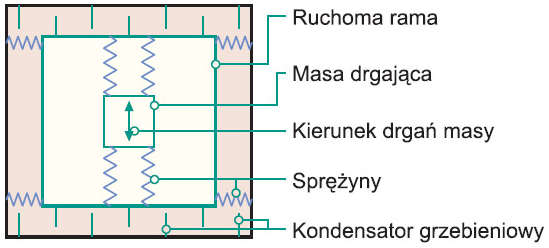
\includegraphics{rys/zyroskopy/kondensator_grzebieniowy}
\par\end{centering}

\caption{Czujnik z kondensatorem grzebieniowym (\emph{�r�d�o:} \cite{elektronikab2b})
\label{fig:kond-grzebien}}


\end{figure}


\begin{figure}
\begin{centering}
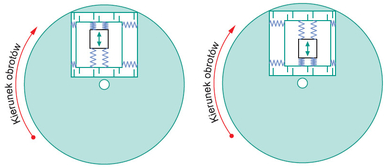
\includegraphics{rys/zyroskopy/zyro_coriolis2}
\par\end{centering}

\caption{�yroskop wibracyjny MEMS z kondensatorem grzebieniowym (\emph{�r�d�o:}
\cite{elektronikab2b}) \label{fig:zyroskop-wibr-mems}}


\end{figure}



\section{�yroskopy wieloosiowe}

Na rysnku dost�pne s� czujniki mierz�ce pr�dko�� obrotow� wok� dw�ch
lub trzech osi. Wcze�niej chc�c uzyska� taki efekt nale�a�o zastosowa�
kilka niezale�nych �yroskop�w jednoosiowych. W wielu zastosowaniach
takie podej�cie si� sprawdza�o, lecz mog�o nie by� optymalne bior�c
pod uwag� koszty oraz miejsce zajmowane przez ca�y uk�ad pomiarowy.
Dzi� problem ten rozwi�zuj� �yroskopy wieloosiowe. Przyk�adowy schematu
blokowy takiego czujnika pokazano na rysunku \ref{fig:czujnik-zyro-dwuosiowy}.
Pr�cz w�a�ciwych �yroskop�w zawiera on tak�e:
\begin{itemize}
\item oscylatory, odpowiedzialne za wprawienie masy w ruch drgaj�cy,
\item uk�ad regulacji amplitudy drga� masy,
\item demodulator synchroniczny,
\item filtr dolnoprzepustowy,
\item pompa �adunkowa odpowiedzialna za wytworzenie wysokiego napi�cia potrzebnego
do zasilenia uk�adu rezonatora pobudzaj�cego mas� do drga�.
\end{itemize}
\begin{figure}
\begin{centering}
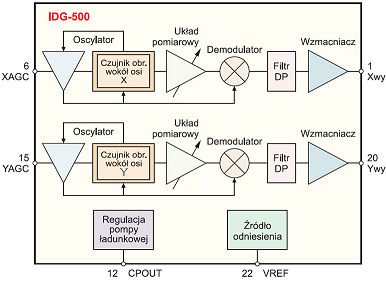
\includegraphics{rys/zyroskopy/zyro_wieloosiowy_schemat}
\par\end{centering}

\caption{Schemat blokowy dwuosiowego czujnika �yroskopowego (\emph{�r�d�o:}
\cite{elektronikab2b}) \label{fig:czujnik-zyro-dwuosiowy}}


\end{figure}



\section{Zastosowania}

\begin{figure}
\begin{centering}
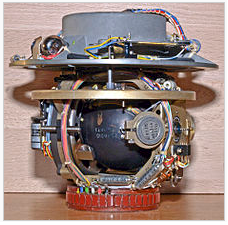
\includegraphics{rys/zyroskopy/zyrokompas}
\par\end{centering}

\caption{�yrokompas (\emph{�r�d�o:} \cite{zyro_wiki})}


\end{figure}


Poni�ej wymieniono niekt�re z praktycznych zastosowa� �yroskop�w:
\begin{itemize}
\item wska�niki komputerowe, myszki, itp.,
\item �yrokompasy u�ywane w nawigacji morskiej,
\item systemy autopilota�u samolot�w,
\item uk�ady utrzymywania orientacji satelit�w,
\item kontrolery gier,
\item uk�ady stabilizacji jednostek p�ywaj�cych,
\item uk�ady detekcji po�o�enia i orientacji w smartfonach i tabletach.\end{itemize}




\chapter{Wsp�praca mikrokontroler�w z urz�dzeniami zewn�trznymi}


\section{Wiadomo�ci og�lne}

\begin{figure}
\begin{centering}
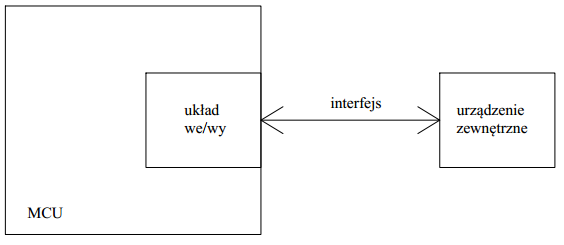
\includegraphics{rys/interfejsy/wspolpraca_z_urz_zew}
\par\end{centering}

\caption{Wsp�praca mikrokontrolera z urz�dzeniem zewn�trznym (\emph{�r�d�o:}
\cite{Krzyzanowski207})}


\end{figure}


Mikrokomputery komunikuj� si� z urz�dzeniami peryferyjnymi poprzez
tzw. interfejsy. Przez interfejs rozumie si� urz�dzenie, kt�re pozwala
na komunikacj� i wymian� danych pomi�dzy dwoma innymi urz�dzeniami.
Istniej� r�ne kryteria podzia�u interfejs�w \cite{Krzyzanowski207}:
\begin{itemize}
\item ze wzgl�du na istnienie fizycznego po��czenia mi�dzy komunikuj�cymi
si� urz�dzeniami:

\begin{itemize}
\item przewodowe (np. UART, I2C, FireWire (IEEE 1394), RS-232), w kt�rych
rol� sygna��w pe�ni� napi�cie lub pr�d, za� rol� medium przewody,
\item bezprzewodowe (np. Bluetooth, IrDA, WiFi), w kt�rych sygna�ami s�
fale elektromagnetyczne, za� medium najcz�ciej powietrze;
\end{itemize}
\item ze wzgl�du na ilo�� danych (bit�w) przesy�anych w trakcie elementarnego
cyklu transmisji:

\begin{itemize}
\item szeregowe (np. SPI, UART, I2C), w kt�rych dane s� transmitowane bit
po bicie,
\item r�wnoleg�e (np. GPIB, SCSI, ATA oraz u�ywany kiedy� w drukarkach interfejs
Centronics);
\end{itemize}
\item ze wzgl�du na charakter sygna��w:

\begin{itemize}
\item analogowe (np. Jack, S-Video),
\item cyfrowe (np. SPI, I2C, USB).
\end{itemize}
\end{itemize}
Pod poj�ciem interfejsu przewodowego rozumie si� z��cza oraz przewody
��cz�ce urz�dzenie zewn�trzne z mikrokomputerem wraz z ich specyfikacj�
mechaniczn� (kszta�t, rozmiar, ilo��) oraz charakterystykami elektrycznymi
sygna��w (poziomy napi�� i pr�d�w, relacje czasowe). Aby przesy� sygna��w
by� mo�liwy, zwi�zany z nimi obw�d elektryczny musi by� zamkni�ty,
dlatego sk�ada si� z dw�ch przewod�w tworz�cych lini�. Istniej� linie
symetryczne i niesymetryczne. Schemat obu pokazano na rysunku \ref{fig:Linie-transmisyjne}.
\begin{figure}
\begin{centering}
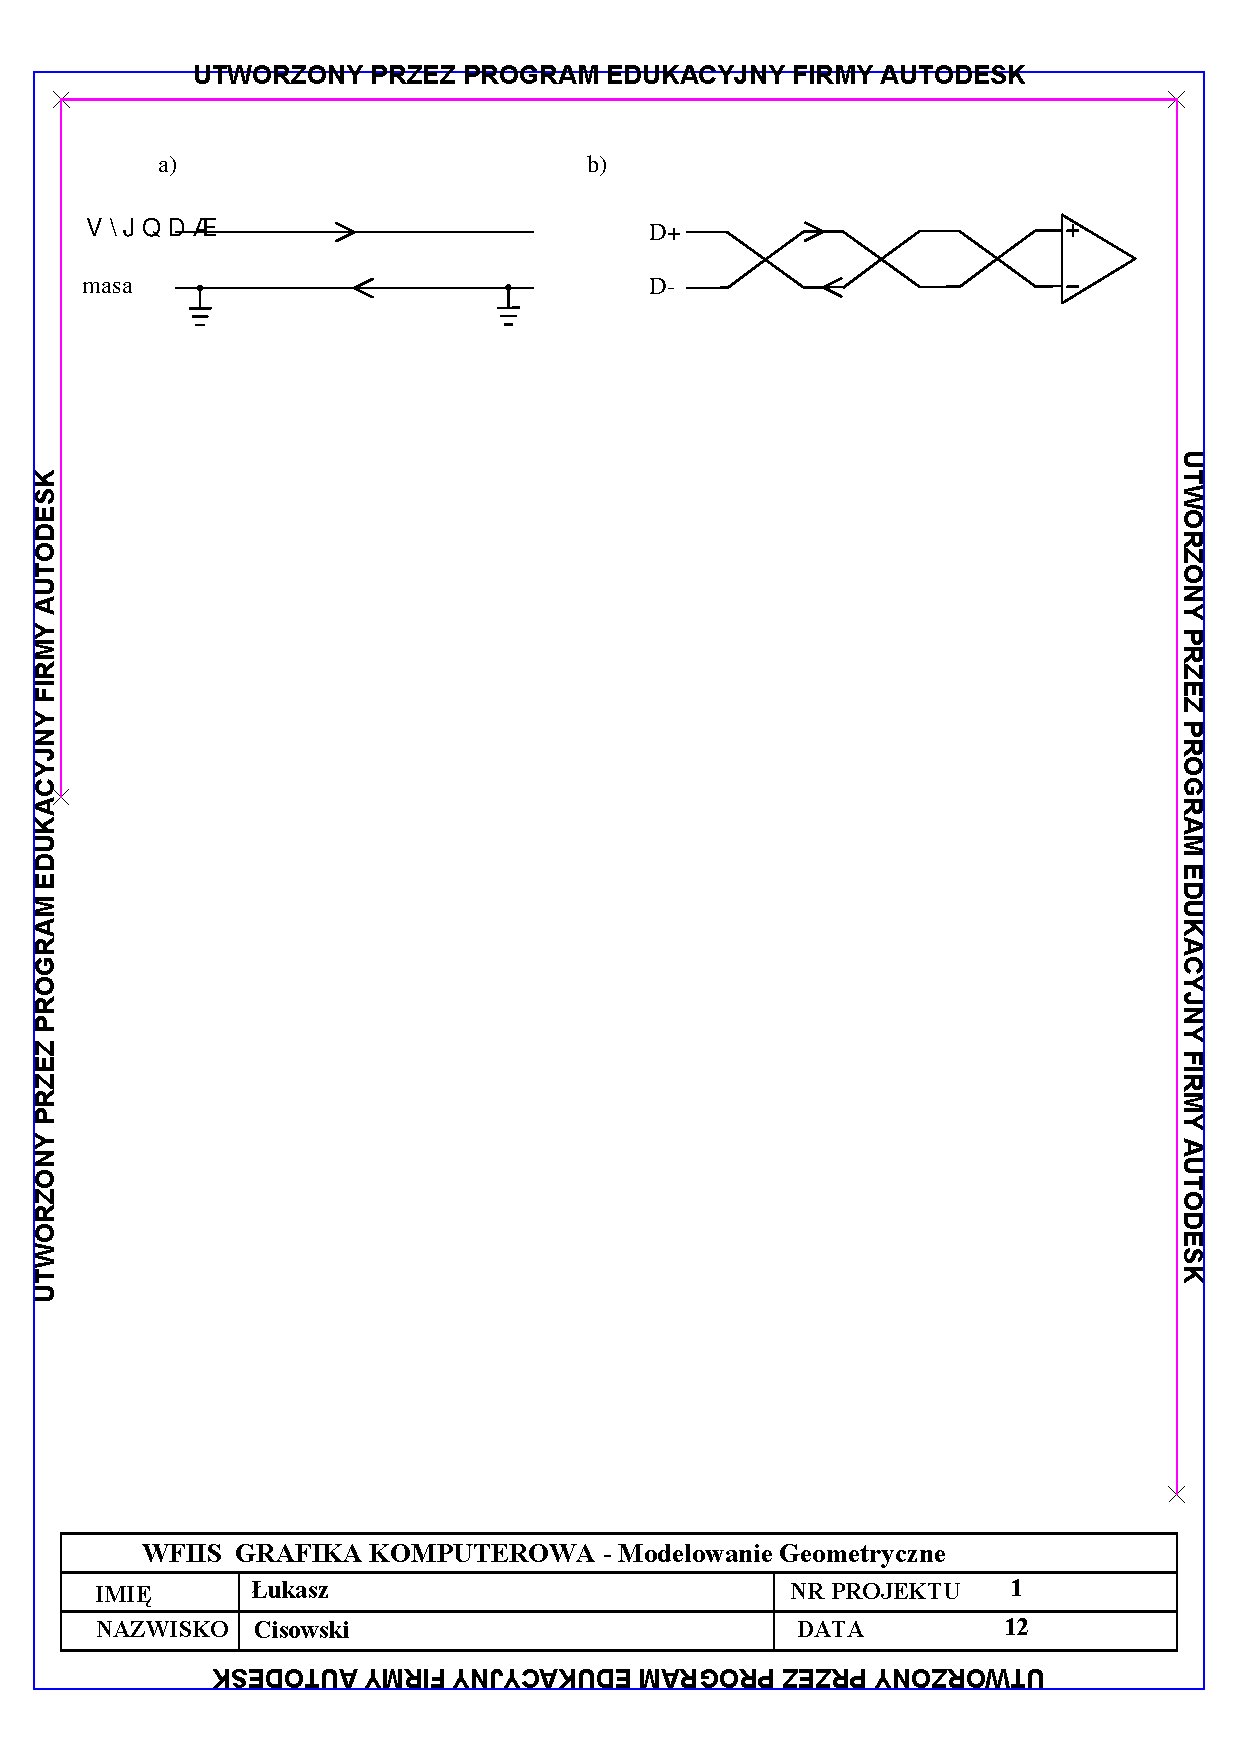
\includegraphics{rys/interfejsy/linie}
\par\end{centering}

\caption{Linie transmisyjne: a) niesymetryczna, b) symetryczna (\emph{�r�d�o:}
\cite{Krzyzanowski207}) \label{fig:Linie-transmisyjne}}


\end{figure}


Linia niesymetryczna sk�ada si� z przewodu sygna�owego (zwanego tak�e
gor�cym) oraz masowego, stanowi�cego referencj� dla sygna�u po obu
stronach toru transmisyjnego. W sytuacji gdy w transmisji u�ywa si�
wi�cej ni� jednego sygna�u, mo�liwe jest zastosowanie wsp�lnego przewodu
powrotnego \cite{Krzyzanowski207}. Linie niesymetryczne s� s�abo
odporne na dzia�anie obcych p�l elektromagnetycznych. Powoduj� one
indukowanie si� zak��ce�, kt�re dodaj� si� lub odejmuj� od w�a�ciwego
sygna�u na wej�ciu odbiornika. Z tego powodu linie tego typu stosuje
si� do przesy�u danych na niedu�e odleg�o�ci. W celu zmniejszenia
wp�ywu zewn�trznych p�l, stosuje si� nast�puj�ce zabiegi:
\begin{itemize}
\item skr�canie przewod�w,
\item ekranowanie linii.
\end{itemize}
Linia symetryczna sk�ada si� z dw�ch przewod�w wiod�cych sygna�y znajduj�ce
si� w przeciwfazie oraz odbiornika z wej�ciem r�nicowym. Dzi�ki temu,
sygna�y o takich samych przebiegach indukowane w~poszczeg�lnych przewodach
znosz� si� po odj�ciu na wej�ciu wzmacniacza. W celu zapewnienia lepszej
ochrony przed zak��ceniami mo�liwe jest r�wnie� skr�canie przewod�w.
Zasi�g linii symetrycznych jest du�o wi�kszy ni� w przypadku linii
niesymetrycznych i osi�ga rz�d 1 km \cite{Krzyzanowski207}.

Najbardziej odpornym na zak��cenia elektromagnetyczne medium jest
�wiat�ow�d. Pozwala on na transmisj� na bardzo du�e odleg�o�ci (od
kilku do kilkudziesi�ciu kilometr�w). Tor �wiat�owodowy wymaga zastosowania
nadajnika przekszta�caj�cego sygna� elektryczny na impulsy �wietlne,
w�a�ciwego �wiat�owodu (wykonanego zwykle z w��kna szklanego) oraz
odbiornika realizuj�cego odwrotn� konwersj� sygna��w.


\subsection{Transmisja szeregowa i r�wnoleg�a}

Transmisja szeregowa polega na przesy�aniu informacji bit po bicie.
Oznacza to, �e w elementarnym cyklu transmisji nadajnik wysy�a jeden
bit, za� odbiornik go odbiera. Zalet� takiego rozwi�zania jest stosunkowo
niewielka ilo�� u�ytych przewod�w. Liczba ta jest wi�ksza w przypadku
transmisji r�wnoleg�ej, w kt�rej na raz mo�liwe jest przesy�anie wi�kszej
ilo�ci bit�w (ka�dy swoim torem). Teoretycznie podnosi to szybko��
transferu danych, jednak w praktyce jest ona ograniczona ze wzgl�du
na zak��canie sygna��w przez pola pochodz�ce od s�siednich linii danych.
Inn� wad� tego typu komunikacji jest tak�e stosunkowo skomplikowana
budowa (a co za tym idzie wi�kszy koszt) interfejs�w r�wnoleg�ych.
Uzasadnia to fakt wykorzystania przez wi�kszo�� wsp�czesnych urz�dze�
cyfrowych interfejs�w i~transmisji szeregowych.

\begin{figure}
\begin{centering}
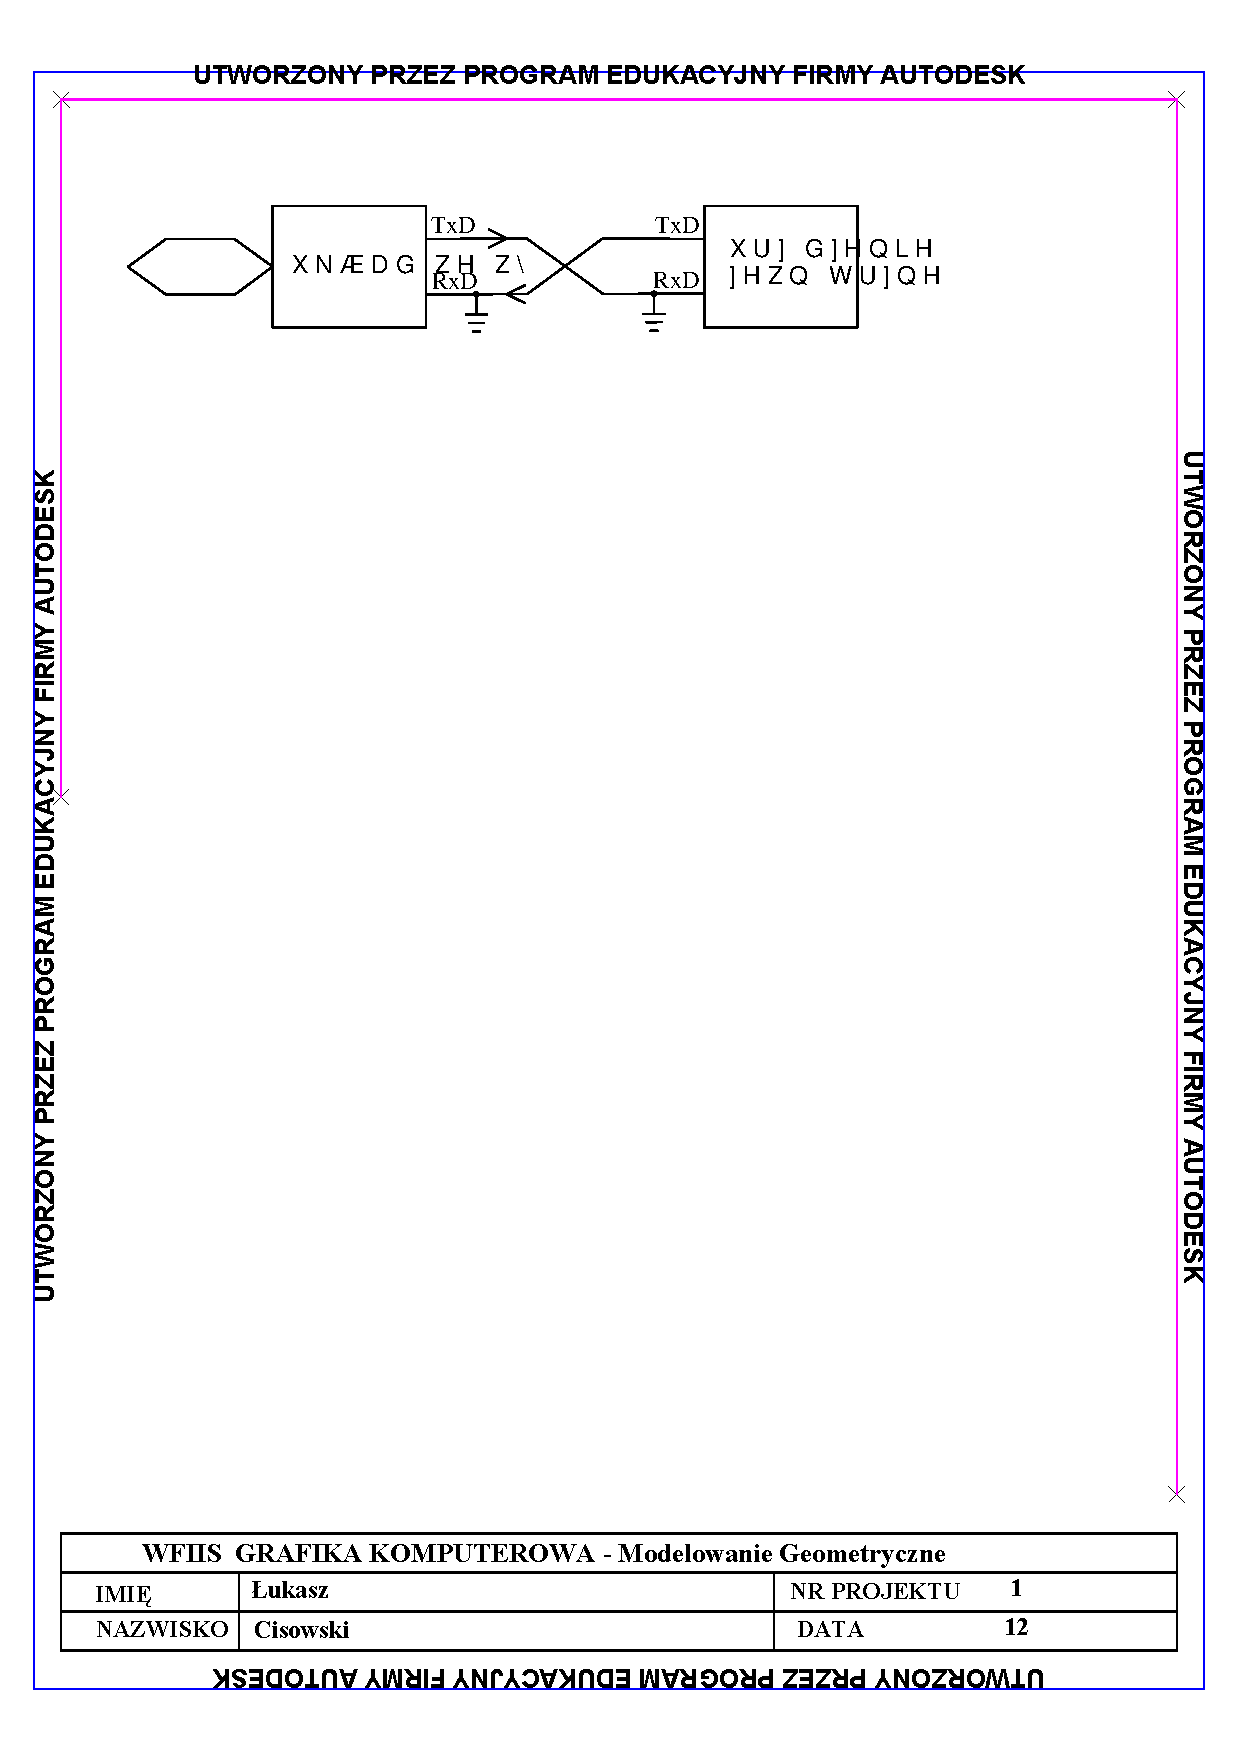
\includegraphics{rys/interfejsy/transmisja_szeregowa}
\par\end{centering}

\caption{Uk�ad transmisji szeregowej (opis sygna��w w tek�cie) (\emph{�r�d�o:}
\cite{Krzyzanowski207}) \label{fig:Uklad-transmisji-szeregowej}}
\end{figure}


Rysunek \ref{fig:Uklad-transmisji-szeregowej} przedstawia uproszczony
schemat uk�adu transmisji szeregowej. Dzi�ki obecno�ci dw�ch przewod�w
sygna�owych, mo�liwa jest komunikacja w trybie dupleks (ang. \emph{full
duplex}), pozwalaj�ca na jednoczesn� wymian� danych przez komunikuj�ce
si� urz�dzenia. Sygna� nadawany (TxD) wysy�any jest do portu odbieraj�cego
dane (RxD). Urz�dzenia uczestnicz�ce w komunikacji wyposa�one s� zar�wno
w nadajnik jak i odbiornik.

Pr�cz transmisji dupleksowej, w uk�adach cyfrowych mo�liwe s� r�wnie�
jeszcze dwa inne tryby wymiany danych:
\begin{itemize}
\item p�dupleks (ang. \emph{half duplex}) -- pozwalaj�cy na obustronn�,
lecz nie jednoczesn� wymian� danych,
\item simpleks (ang. \emph{simplex}) -- pozwalaj�cy na przesy� danych tylko
w jednym kierunku.
\end{itemize}
Dane wysy�ane szeregowo s� cz�sto przechowywane w rejestrach. Aby
umo�liwi� transmisj� bit po bicie stosuje si� rejestry przesuwne lub
multipleksery. W obu przypadkach nale�y zdefiniowa� czas transmisji
pojedynczego bitu \cite{Krzyzanowski207}. S�u�y do tego sygna� zegarowy
nadajnika. Odbiornik okre�la warto�� danego bitu w po�owie czasu jego
trwania. Istniej� dwa rodzaje transmisji szeregowej:
\begin{itemize}
\item transmisja asynchroniczna,
\item transmisja synchroniczna.
\end{itemize}

\subsection{Transmisja asynchroniczna i synchroniczna}

W przypadku transmisji asynchronicznej zegary nadajnika i odbiornika
nie s� synchronizowane. Dane nie musz� by� przesy�ane w spos�b ci�g�y,
tzn. mi�dzy kolejnymi transmisjami, linia danych znajduje si� w stanie
spoczynku przez tzw. czas martwy. Dane przesy�ane nosz� tak�e nazw�
znaku i~zawieraj� zwykle od pi�ciu do o�miu bit�w. Aby odbiornik
m�g� wykry� pocz�tek oraz koniec nadawania danych, ka�dy znak poprzedzony
jest tzw. bitem startu oraz zako�czony tzw. bitami stopu (od jednego
do dw�ch). Dodatkowo w celu zapewnienia poprawno�ci transmisji stosuje
si� r�wnie� tzw. bit parzysto�ci. Wad� transmisji asynchronicznej
jest istnienie czasu martwego, zmniejszaj�cego efektywno�� przesy�u
danych. Suma liczby jedynek tworz�cych znak wraz z bitem parzysto�ci
powinna tworzy� liczb� parzyst�.

\begin{figure}
\begin{centering}
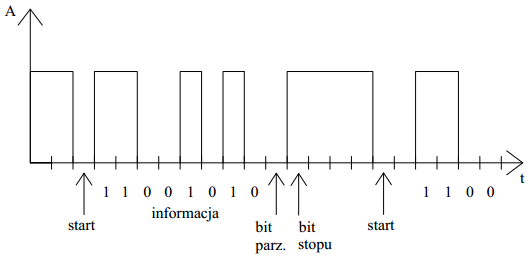
\includegraphics{rys/interfejsy/transmisja_szeregowa_asynchroniczna}
\par\end{centering}

\caption{Przebieg sygna�u w transmisji szeregowej asynchronicznej (\emph{�r�d�o:}
\cite{Krzyzanowski207})}


\end{figure}


Przed w�a�ciw� komunikacj� nale�y ustali� jej nast�puj�ce parametry:
\begin{itemize}
\item cz�stotliwo�� zegar�w,
\item d�ugo�� znaku,
\item bit parzysto�ci (obecny, nieobecny lub zanegowany),
\item ilo�� bit�w stopu.
\end{itemize}
W transmisji synchronicznej, wsp�lny sygna� zegarowy przesy�any jest
dodatkow� lini�, dzi�ki czemu zar�wno odbiornik jak i nadajnik przesy�aj�
bity w jednakowych odst�pach czasu. Dane zgrupowane s� w bloki zwane
ramkami (ang. \emph{frame}). Ka�d� ramk� rozpoczyna nag��wek (rysunek
\ref{fig:Ramka-transmisji-szeregowej-synchr}), zawieraj�cy dodatkowe
informacje, np. ilo�� przesy�anych danych. Blok danych zawiera w�a�ciwe
dane zgrupowane jeden za drugim. W celu zapewnienia poprawno�ci transmisji,
s� one zako�czone tzw. bajtami kontrolnymi i ewentualnymi bajtami
korekcyjnymi pozwalaj�cymi na napraw� uszkodzonych danych \cite{Krzyzanowski207}.

\begin{figure}
\begin{centering}
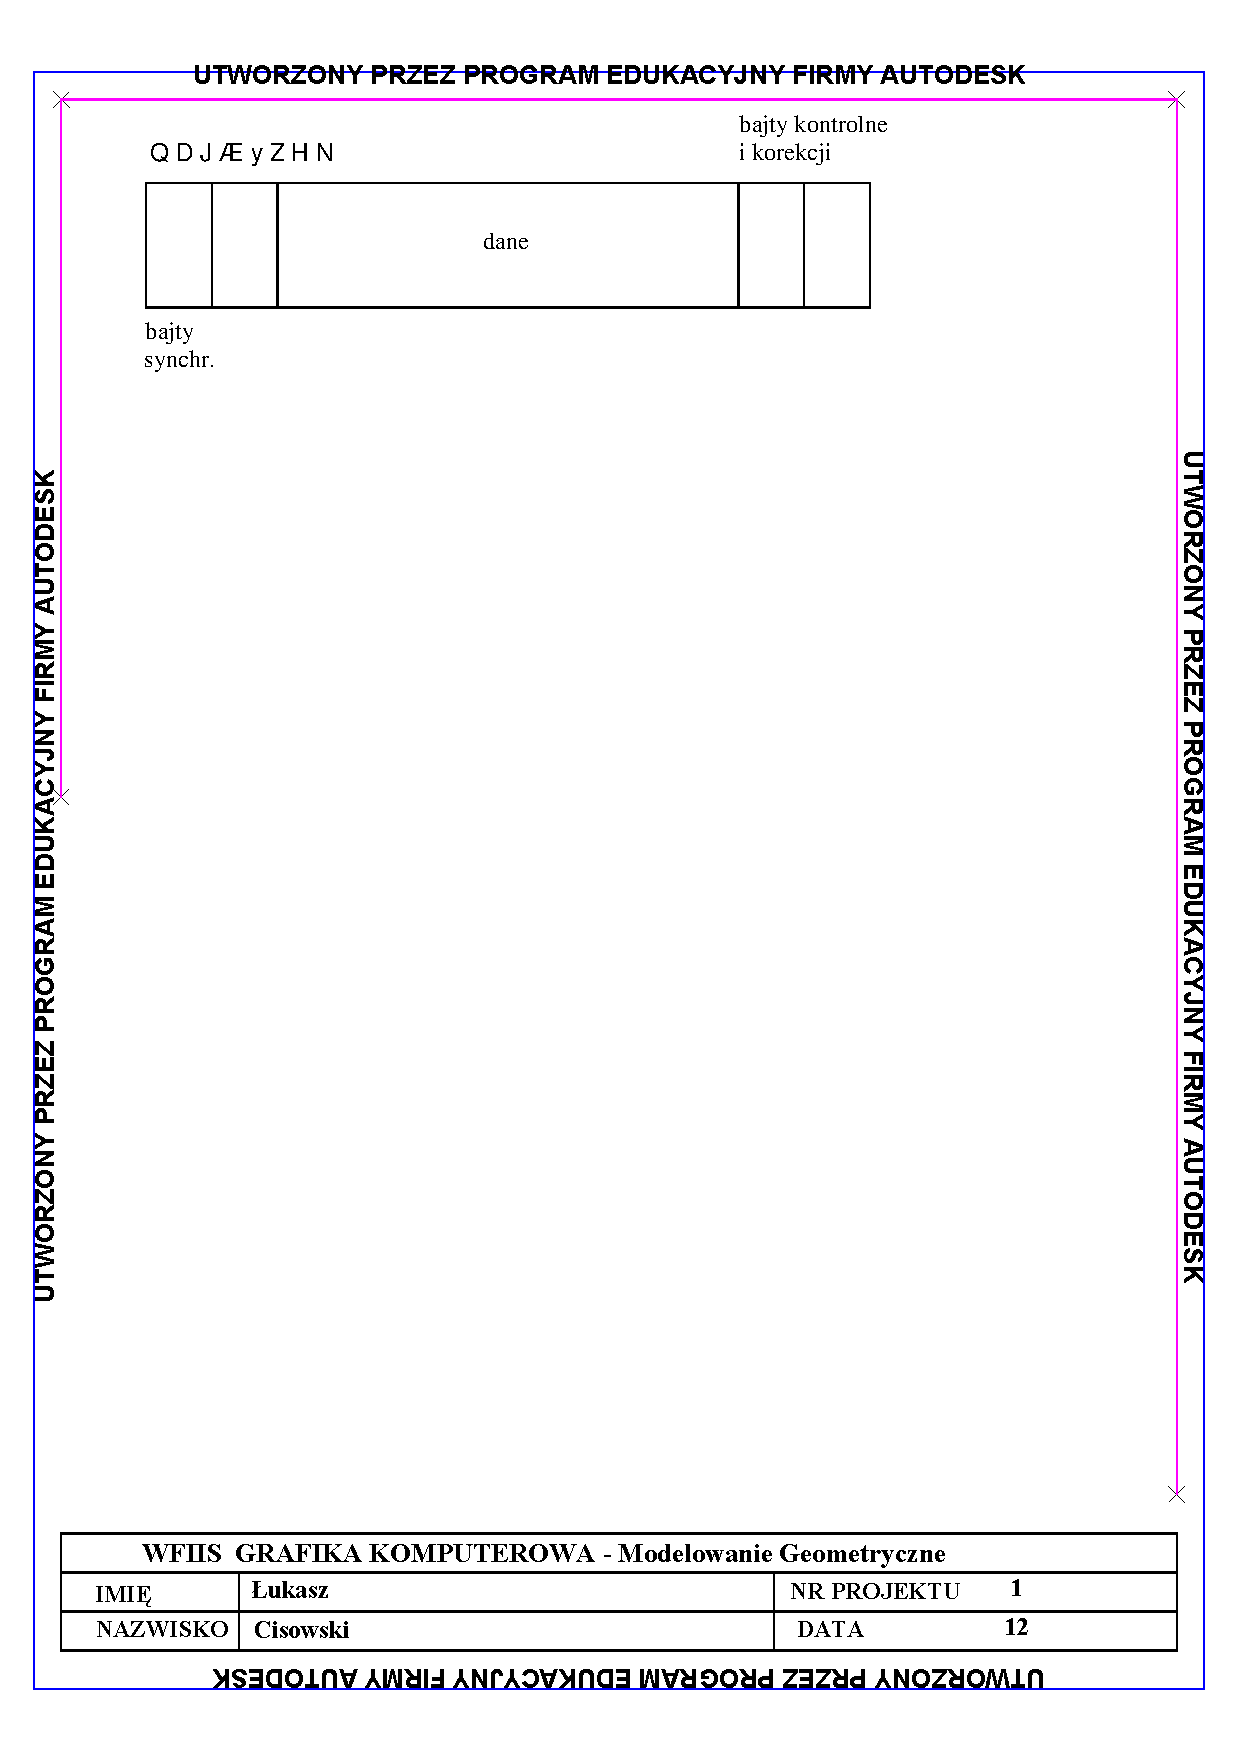
\includegraphics{rys/interfejsy/ramka_transmisji_szeregowej_synchronicznej}
\par\end{centering}

\caption{Ramka transmisji szeregowej synchronicznej (\emph{�r�d�o:} \cite{Krzyzanowski207})
\label{fig:Ramka-transmisji-szeregowej-synchr}}


\end{figure}



\subsection{Interfejsy typu \textit{master} -- \emph{slave}\label{sub:Interfejsy-typu-master}}

Jest to model komunikacji, w kt�rym jedno z kilku urz�dze� pe�ni rol�
nadrz�dnego w stosunku do pozosta�ych. Urz�dzenie nadrz�dne nazywane
jest \emph{master}'em, podczas gdy pozosta�e uk�ady to \emph{slave}'y.
Rol� \emph{master}'a jest kontrola ca�ego procesu komunikacji. Urz�dzenie
nadrz�dne inicjalizuje komunikacj� ze \emph{slave}'ami i kontroluje
ich dzia�anie. Jedynym typem danych przep�ywaj�cym w odwrotnym kierunku
s� odpowiedzi urz�dze� podrz�dnych na otrzymane zapytania. Interfejsy
tego typu s� powszechnie stosowane w technice ze wzgl�du na du�� niezawodno��
komunikacji i wzgl�dn� prostot� dzia�ania. Przyk�adami tego typu komunikacji
mog� by� interfejsy takie jak: SPI, I\textsuperscript{2}C, 1-Wire,
Modbus i wiele innych.


\section{Interfejs SPI}

Interfejs SPI (ang. \emph{Serial Peripheral Interface}) zosta� zaprojektowany
i po raz pierwszy zastosowany przez firm� Motorola. Jest jednym z
najcz�ciej u�ywanych interfejs�w mi�dzy mikroprocesorami a~urz�dzeniami
zewn�trznymi takimi jak przetworniki A/D oraz D/A, pami�ci EEPROM,
czujniki (akcelerometry, �yroskopy), pami�ci flash, sterowniki ekran�w
dotykowych itp. W �wietle om�wionych wcze�niej cech interfejs�w, SPI
mo�e by� scharakteryzowany jako:
\begin{itemize}
\item szeregowy,
\item synchroniczny,
\item komunikuj�cy si� w trybie \emph{full duplex},
\item przewodowy.
\end{itemize}
Komunikacja z urz�dzeniami wykonywana jest w oparciu o opisany w rozdziale
\ref{sub:Interfejsy-typu-master} model wymiany danych \emph{master}
- \emph{slave}. Do przesy�u danych wykorzystywane s� zwykle 4 przewody,
cho� interfejs mo�e r�wnie� funkcjonowa� w postaci tr�jprzewodowej.
SPI jest standardem \emph{de facto}, tzn. jest powszechnie stosowany
przez wielu producent�w sprz�tu elektronicznego, lecz w przeciwie�stwie
do standardu \emph{de jure} nie istnieje jego formalna specyfikacja
zaakceptowana przez komitety standaryzacyjne typu IEEE, ANSI lub ISO.
Interfejs SPI jest te� czasem okre�lany jako czteroprzewodowa magistrala
szeregowa lub SSI (ang. \emph{Synchronous Serial Interface}).

Omawiany interfejs obejmuje cztery sygna�y:
\begin{itemize}
\item sygna� zegarowy SCLK (wyj�cie urz�dzenia\emph{ master}),
\item sygna� MOSI (ang. \emph{Master Output Slave Input}) -- wyj�cie urz�dzenia
\emph{master} i wej�cie urz�dzenia \emph{slave},
\item sygna� MISO (ang. \emph{Master Input Slave Output}) -- wej�cie urz�dzenia
\emph{master} i wyj�cie urz�dzenia \emph{slave},
\item sygna� CS (ang. \emph{Chip Select}) lub SS (ang. \emph{Slave Select})
-- sygna� wyboru urz�dzenia (wyj�cie urz�dzenia \emph{master}).
\end{itemize}
Wymienione powy�ej sygna�y posiadaj� tak�e alternatywne nazwy:
\begin{itemize}
\item SCLK -- SCK, CLK,
\item MOSI -- SIMO, SDO, DO,
\item MISO -- SOMI, SDI, DI,
\item CS -- nCS, nSS, CSB, STE.
\end{itemize}

\subsection{Przesy� danych}

\begin{figure}
\begin{centering}
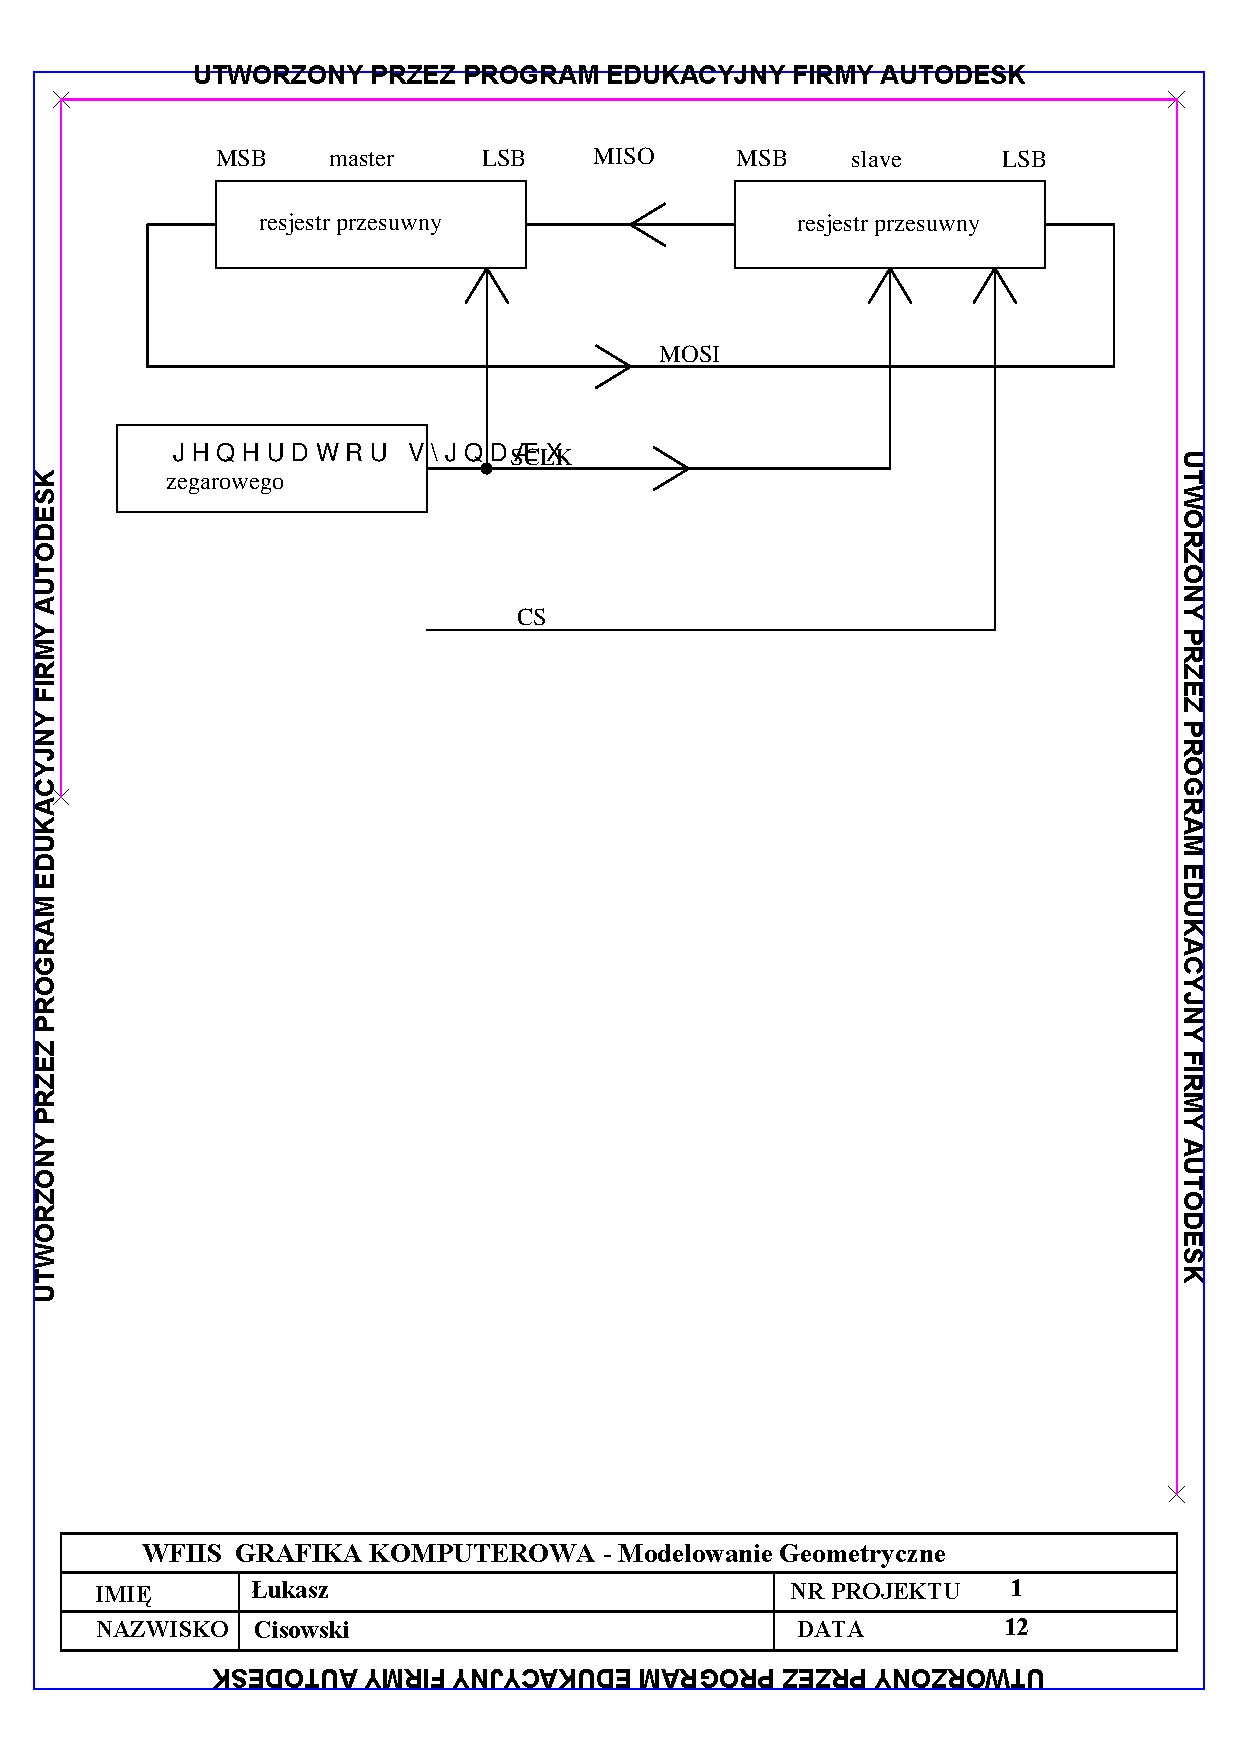
\includegraphics{rys/interfejsy/spi_rejestry_przesuwne}
\par\end{centering}

\caption{Typowa realizacja transmisji SPI przy pomocy cyklicznego rejestru
przesuwnego (\emph{�r�d�o:} \cite{spi_am_gdynia}) \label{fig:spi-rej-przesuwny}}


\end{figure}


Przed dokonaniem transmisji danych, urz�dzenie \emph{master} musi
okre�li� odpowiedni� cz�stotliwo�� sygna�u zegarowego. Nie mo�e by�
ona wi�ksza od �adnej z maksymalnych dopuszczalnych cz�stotliwo�ci
wspieranych przez urz�dzenia \emph{slave}. Nast�pnie sygna� wyboru
urz�dzenia (CS) przechodzi w stan aktywny (zwykle logiczne 0). Je�li
nale�y poczeka�, aby wsp�pracuj�ce urz�dzenie podrz�dne dokona�o
przetwarzania danych (tak jest np. w przypadku przetwornik�w analogowo-cyfrowych),
urz�dzenie nadrz�dne musi wstrzyma� si� z generacj� sygna�u zegarowego.

Z ka�dym taktem zegara zwi�zany jest cykl komunikacji \emph{full duplex}:
\begin{itemize}
\item urz�dzenie master wysy�a lini� MOSI kolejny bit, za� slave go odbiera,
\item urz�dzenie slave wysy�a kolejny bit danych lini� MISO, za� master
go odbiera.
\end{itemize}
W transmisji wykorzystywane s� zwykle dwa rejestry przesuwne (po jednym
dla urz�dzenia master i~slave) po��czone ze sob� tworz�c rejestr
cykliczny (rysunek \ref{fig:spi-rej-przesuwny}). Zwykle wysy�any
jest najbardziej znacz�cy bit MSB (ang. \emph{most significant bit})
a odbierany najmniej znacz�cy LSB (ang. \emph{least significant bit}).
Po wype�nieniu rejestr�w nast�puje obr�bka zawartych w nich danych,
tj. zapis do pami�ci, przetwarzanie itp. W celu wymiany wi�kszej ilo�ci
informacji, wspomniany proces si� powtarza. W trakcie pojedynczego
cyklu komunikacji przesy�any jest zwykle bajt danych (8 bit�w), cho�
nie jest to regu��; istniej� uk�ady w kt�rych przesy�a si� 12 lub
16 bit�w. Niekt�re urz�dzenia \emph{slave} nie pozwalaj� na odbieranie
danych w ci�gu wi�kszej od zadanej liczby takt�w sygna�u zegarowego;
w innych rozwi�zaniach konstrukcyjnych dane nadmiarowe s� ignorowane.

Opr�cz wymienionych sygna��w steruj�cych komunikacj�, w urz�dzeniu
\emph{slave} mo�liwe jest r�wnie� wyprowadzenie sygna�u przerwania.
Przyk�adowo mo�e to by� sygna� informuj�cy o dotkni�ciu ekranu dotykowego,
sygna� alarmowy generowany przez czujnik temperatury lub zegar czasu
rzeczywistego. Standard SPI nie przewiduje u�ycia przerwa�, chocia�
przeznaczanie dla nich oddzielnego pinu w~urz�dzeniu \emph{slave}
nie jest ani zakazane ani obowi�zkowe.

�adne z urz�dze� \emph{slave}, kt�re nie zosta�o aktywowane sygna�em
CS nie powinno reagowa� na sygna� taktuj�cy ani sterowa� wsp�ln� magistral�.
Urz�dzenie \emph{master}, wybiera za� do wymiany informacji tylko
jedno urz�dzenie podrz�dne.


\subsection{Faza i polaryzacja sygna�u zegarowego}

\begin{figure}
\begin{centering}
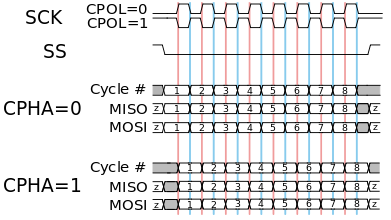
\includegraphics{rys/interfejsy/spi_pol_faza}
\par\end{centering}

\caption{Przebiegi odpowiadaj�ce r�nym polaryzacjom i fazom sygna�u taktuj�cego
(\emph{�r�d�o:} \cite{spi_pol_ph})}


\end{figure}


Poza okre�leniem cz�stotliwo�ci sygna�u taktuj�cego, urz�dzenie nadrz�dne
musi tak�e zdefiniowa� polaryzacj� i faz� tego sygna�u. Zwykle jest
to zwi�zane z wpisaniem do odpowiednich rejestr�w konfiguracyjnych
warto�ci 0 lub 1 na odpowiednich pozycjach. Bity na tych pozycjach
zwykle nazywane s� CPOL (dla okre�lenia polaryzacji) oraz CPHA (dla
okre�lenia fazy); ich znaczenie jest nast�puj�ce:
\begin{itemize}
\item je�li CPOL = 0, to stanem nieaktywnym sygna�u zegara jest stan niski
oraz:

\begin{itemize}
\item je�li CPHA = 0, to dane zapisywane s� przy zboczu narastaj�cym zegara,
za� przesy�ane przy opadaj�cym,
\item je�li CPHA = 1, to dane zapisywane s� przy zboczu opadaj�cym zegara,
za� przesy�ane przy narastaj�cym,
\end{itemize}
\item je�li CPOL = 1, to stanem nieaktywnym sygna�u taktuj�cego jest stan
wysoki oraz:

\begin{itemize}
\item je�li CPHA = 0, to dane zapisywane s� przy zboczu opadaj�cym zegara,
za� przesy�ane przy narastaj�cym,
\item je�li CPHA = 1, to dane zapisywane s� przy zboczu narastaj�cym zegara,
za� przesy�ane przy opadaj�cym.
\end{itemize}
\end{itemize}

\subsection{Wsp�praca z kilkoma urz�dzeniami podrz�dnymi}

Jak wspomniano wcze�niej, interfejs SPI pozwala na wsp�prac� jednego
urz�dzenia nadrz�dnego z kilkoma urz�dzeniami \emph{slave}. Jednym
ze sposob�w zorganizowania takiego uk�adu transmisji danych jest zastosowanie
niezale�nych sygna��w CS dla ka�dego z urz�dze� podrz�dnych. Przyk�ad
takiego rozwi�zania pokazano na rysunku \ref{fig:spi-independent-slaves}.
Poniewa� wszystkie wyj�cia MISO uk�ad�w \emph{slave} s� po��czone
do wsp�lnej linii, powinny by� one wyj�ciami tr�jstanowymi.

\begin{figure}
\begin{centering}
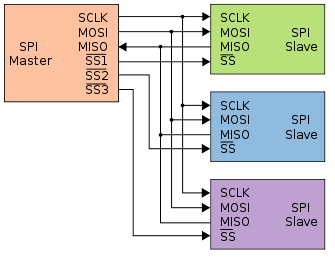
\includegraphics{rys/interfejsy/spi_independent_slaves}
\par\end{centering}

\caption{Typowa realizacja komunikacji przy pomocy interfejsu SPI z wieloma
urz�dzeniami \emph{slave} (\emph{�r�d�o:} \cite{spi_independent_slaves})
\label{fig:spi-independent-slaves}}


\end{figure}


Niekt�re urz�dzenia wspieraj�ce SPI s� zaprojektowane z my�l� o zastosowaniu
po��czenia �a�cuchowego (znanego w literaturze angloj�zycznej jako
\emph{daisy chain}). W takiej konfiguracji wyj�cie jednego z~urz�dze�
\emph{slave} jest po��czone do wej�cia drugiego \emph{slave'a} itd.
Port SPI takiego urz�dzenia podrz�dnego w danym cyklu transmisji odbiera
dane od poprzedniego urz�dzenia, kt�re te same dane odebra�o w~poprzednim
cyklu. Ca�a kaskada dzia�a jak jeden du�y rejestr przesuwny. Zalet�
takiego rozwi�zania jest to, �e urz�dzenie typu \emph{master} mo�e
wykorzystywa� tylko jeden sygna� CS. Schemat takiego po��czenia przedstawiono
na rysunku \ref{fig:Komunikacja-przy-pomocy}.

\begin{figure}
\begin{centering}
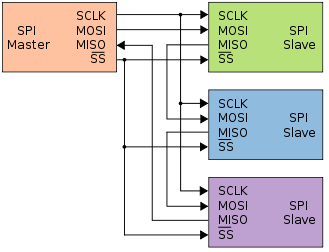
\includegraphics{rys/interfejsy/spi_daisy_chain}
\par\end{centering}

\caption{Komunikacja przy pomocy interfejsu SPI w konfiguracji \emph{daisy
chain} (\emph{�r�d�o:} \cite{spi_daisy_chain})\label{fig:Komunikacja-przy-pomocy}}


\end{figure}



\subsection{Zalety i wady interfejsu SPI}

Do zalet interfejsu SPI mo�emy zaliczy�:
\begin{itemize}
\item komunikacja w trybie \emph{full duplex},
\item ilo�� przesy�anych danych nie jest ograniczona do 8 bit�w,
\item prosty do zrozumienia i implementacji protok�,
\item stosunkowo prosta budowa:

\begin{itemize}
\item relatywnie ma�o skomplikowane obwody elektryczne, mniejsze zu�ycie
energii,
\item urz�dzenia \emph{slave} u�ywaj� wsp�lnego sygna�u zegarowego generowanego
przez uk�ad \emph{master} (dodatkowe precyzyjne oscylatory i p�tle
PLL s� niepotrzebne),
\item urz�dzenia slave nie wymagaj� unikalnych adres�w (w przeciwie�stwie
do I2C, GPIB czy SCSI),
\item nie s� wymagane transceivery,
\end{itemize}
\item wystarczaj� tylko 4 piny,
\item wi�kszo�� linii sygna�owych mo�e by� wsp�dzielonych przez r�ne urz�dzenia
\emph{slave}.
\end{itemize}
W�r�d wad interfejsu SPI mo�na wymieni�:
\begin{itemize}
\item wi�ksz� w por�wnaniu do I\textsuperscript{2}C ilo�� pin�w obudowy
IC,
\item brak sprz�towej kontroli przep�ywu danych przez urz�dzenia \emph{slave},
\item brak sprz�towego potwierdzania obecno�ci urz�dzenia \emph{slave} (\emph{master}
mo�e ,,rozmawia�'' z niczym),
\item brak wsparcia dla architektury multi-master,
\item brak oficjalnego standardu,
\item brak protoko�u obs�ugi b��d�w,
\item brak wsparcia dla dynamicznego pod��czania urz�dze� \emph{slave},
\item dzia�anie na stosunkowo niedu�e odleg�o�ci.
\end{itemize}

\subsection{Zastosowania}

Du�o mniejsza w por�wnaniu z interfejsami r�wnoleg�ymi liczba niezb�dnych
pin�w powoduje, �e SPI jest bardzo cz�sto wykorzystywany w systemach
wbudowanych. Jest on elementem wielu mikrokontroler�w z rodziny ARM,
AVR, PIC oraz MSP. Niekt�re mikrokontrolery AVR mog� by� programowane
z u�yciem interfejsu SPI. Cz�sto u�ywa si� go tak�e do komunikacji
z takimi uk�adami peryferyjnymi jak:
\begin{itemize}
\item czujniki temperatury, ci�nienia, przyspieszenia,
\item przetworniki ADC oraz DAC,
\item kontrolery ekran�w dotykowych oraz gier,
\item pami�ci flash oraz EEPROM,
\item zegary RTC,
\item karty MMC oraz SD.
\end{itemize}

\section{Interfejs UART\label{sec:Interfejs-UART}}

UART (ang. \emph{Universal Asynchronous Receiver and Transmitter})
jest protoko�em umo�liwiaj�cym asynchroniczne odbieranie i nadawanie
informacji przy pomocy portu szeregowego. Sk�ada si� z trzech zasadniczych
element�w:
\begin{itemize}
\item konwertera r�wnoleg�o-szeregowego (ang. \emph{parallel to serial}),
pozwalaj�cego na przesy�anie danych z urz�dzenia cyfrowego (komputer,
mikrokontroler itp.),
\item konwertera szeregowo-r�wnoleg�ego, umo�liwiaj�cego odbi�r danych przez
urz�dzenie cyfrowe (np. komputer lub mikrokomputer),
\item bufora danych, gromadz�cego tymaczasowo dane w przypadku szybkiej
komunikacji.
\end{itemize}
UART u�ywany jest cz�sto w po��czeniu z takim standardami komunikacyjnymi
jak RS-232, EIA czy RS-485. Jego uniwersalno�� polega na tym, �e szybko��
transmisji oraz format danych s� konfigurowalne. Poziomy elektryczne
sygna��w elektrycznych oraz ich posta� (np. sygna� r�nicowy) ustawiane
s� przez zewn�trzny uk�ad sterownika. Omawiane urz�dzenia wyst�puj�
jako uk�ady scalone (b�d� ich komponenty) b�d�ce sk�adnikami mikrokontroler�w.
Istniej� konstrukcje ��cz�ce dwa (DUART) lub osiem uk�ad�w UART w
jednej obudowie. Istniej� r�wnie� chipy pozwalaj�ce na komunikacj�
synchroniczn�, okre�lane w skr�cie jako USART (ang. \emph{Universal
Synchronous and Asynchronous Receiver and Transmitter}).


\subsection{Transmisja}

Uniwersalny asynchroniczny odbiornik/nadajnik przesy�a bajty danych
bit po bicie. UART znajduj�cy si� po drugiej stronie odbiera poszczeg�lne
bity ��cz�c je w bajty. Konwersj� z r�wnoleg�ej postaci danych na
szeregow� uzyskuje si� zwykle przy pomocy rejestr�w przesuwnych b�d�cych
sk�adnikami UART�w. U�ycie szeregowej transmisji danych zamiast r�wnoleg�ej
(bardziej naturalnej dla urz�dze� cyfrowych) pozwala na zmniejszenie
koszt�w oraz problem�w zwi�zanych z zak��ceniami elektromagnetycznymi.

UART zwykle nie generuje ani nie odbiera bezpo�rednio sygna��w odpowiedzialnych
za komunikacj�. W tym celu u�ywa si� dodatkowych interfejs�w, konwertuj�cych
sygna�y u�ywane przez UART na w�a�ciwe przebiegi odpowiadaj�ce za
transmisj� danych. Cz�sto u�ywanymi standardami s� RS-232, RS-485
oraz EIA. Komunikacja mo�e odbywa� si� w trybie \emph{simplex}, \emph{half
duplex} oraz \emph{full duplex}.


\subsection{Ramka danych}

\begin{figure}
\begin{centering}
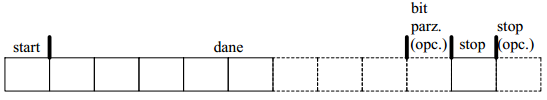
\includegraphics{rys/interfejsy/ramka_uart}
\par\end{centering}

\caption{Ramka danych wysy�ana lub odbierana przez UART \label{fig:Ramka-danych-uart}}


\end{figure}


Rysunek \ref{fig:Ramka-danych-uart} przedstawia typow� ramk� u�ywane
w trakcie transmisji przy pomocy uk�adu UART. W stanie bezczynno�ci
(gdy nie przesy�ane s� �adne dane), linia danych jest zwykle w stanie
wysokim. Wysy�anie w�a�ciwych danych (zwanych znakiem) sygnalizowane
jest bitem startu, tj. przej�ciem linii danych do stanu niskiego.
Przesy�any znak sk�ada si� zazwyczaj z 5 - 8 bit�w. W celu zapewnienia
kontroli poprawno�ci danych, mo�e by� zako�czony tzw. bitem parzysto�ci.
W celu zasygnalizowania odbiornikowi zako�czenia transmisji, przesy�any
jest bit stopu, kt�ry mo�e by� zdublowany.


\subsection{Odbi�r danych}

Wszystkie operacje w uk�adzie UART sterowane s� sygna�em zegarowym
o cz�stotliwo�ci b�d�cej wielokrotno�ci� cz�sto�ci u�ywanej do przesy�ania
danych. Odbiornik pr�bkuje lini� danych w oczekiwaniu na pojawienie
si� bitu startu. Je�li linia danych przejdzie ze stanu spoczynkowego
do aktywnego na czas wynosz�cy co najmniej po�ow� okresu trwania bitu,
zostanie to zinterpretowane jako bit startu. W~przeciwnym wypadku
zarejestrowany impuls zostanie zignorowany. Nast�pnie po up�ywie niewielkiego
czasu nast�puje dalsze pr�bkowanie linii danych po��czone z wczytywaniem
znaku do odbiorczego rejestru przesuwnego. Po wczytaniu okre�lonej
liczby bit�w, UART ustawia odpowiedni� flag� lub generuje sygna� przerwania
informuj�cy mikroprocesor o odebraniu danych.

Komunikuj�ce si� uk�ady UART nie posiadaj� wsp�lnego sygna�u zegarowego.
Ka�dy z nich posiada w�asne zegary, kt�rych synchronizacja dokonuje
si� w oparciu o sygna� na linii danych. Zwykle synchronizacja ma miejsce
w chwili zmiany stanu linii danych, o ile zmiana ta mo�e by� uznana
za wa�n�. Uproszczone uk�ady synchronizuj� si� w momencie detekcji
opadaj�cego zbocza bitu startu, za� odczyt kolejnych bit�w nast�puje
w po�owach czas�w ich trwania. Takie rozwi�zanie dzia�a poprawnie,
o ile szybko�� transmisji pozwala na poprawny odczyt bit�w stopu.

Standardow� cech� uk�ad�w UART jest pobieranie kolejnego znaku, gdy
poprzedni zosta� zapisany w rejestrze. Zastosowane w ten spos�b podw�jne
buforowanie pozwala mikroprocesorowi na odczyt poprzedniego znaku,
przed odebraniem nast�pnego. Je�li centralna jednostka przetwarzaj�ca
po stronie odbiornika potrzebuje jeszcze wi�cej czasu na odbi�r, mo�na
zastosowa� buforowanie danych z u�yciem kolejek FIFO.


\subsection{Nadawanie danych}

Po umieszczeniu znaku w rejestrze przesuwnym nadajnika, UART wysy�a
na lini� danych bit startu, kolejne bity danych, bit parzysto�ci (je�li
jest u�ywany) oraz bit (lub dwa bity) stopu. Poniewa� transmisja pojedynczego
znaku zajmuje pewien czas, uk�ad nadawczy ustawia odpowiedni� flag�
zaj�to�ci, kt�ra informuje mikroprocesor, �eby nie umieszcza� kolejnego
znaku w rejestrze przesuwnym. Zamiast flagi mo�e by� wygenerowane
odpowiednie przerwanie. W przypadku trybu \emph{full duplex} oba uk�ady
UART u�ywaj� dw�ch rejestr�w przesuwnych.


\subsection{W�asno�ci}

Oba uk�ady UART, zar�wno nadawczy jak i odbiorczy musz� mie� zgodne
nast�puj�ce parametry:
\begin{itemize}
\item szybko�� transmisji danych,
\item ilo�� bit�w danych,
\item obecno�� (lub jej brak) bitu parzysto�ci,
\item ilo�� bit�w stopu.
\end{itemize}
W przypadku niezgodno�ci ww. parametr�w, uk�ad odbiorczy mo�e ustawi�
odpowiedni� flag� b��du. Typowo porty szeregowe komputer�w wykorzystuj�
osiem bit�w danych, bit parzysto�ci i jeden bit stopu.


\subsection{Transmisja w trybie synchronicznym}

Jak wspomniano wcze�niej istniej� uk�ady typu USART potrafi�ce tak�e
pracowa� w trybie transmisji synchronicznej. W tym wypadku przebieg
sygna�u zegarowego jest pozyskiwany na podstawie sygna�u na linii
danych. Dzi�ki obecno�ci sygna�u synchronizacyjnego niepotrzebne staj�
si� bity startu i~stopu, co pozwala na lepsze wykorzystanie linii
danych i w efekcie bardziej efektywn� komunikacj�. W~przypadku trybu
asynchronicznego, gdy nie ma danych do przes�ania, linia danych znajduje
si� w stanie spoczynku. W trybie transmisji synchronicznej konieczne
jest przesy�anie specjalnych znak�w w celu utrzymania synchronizacji.


\subsection{Stany b��dne}

Poni�ej opisano mo�liwe b��dy towarzysz�ce komunikacji z wykorzystaniem
urz�dze� UART.
\begin{itemize}
\item B��d przepe�nienia (ang. \emph{overrun error}) -- wyst�puje, gdy odbiorca
nie mo�e przetworzy� jednej porcji danych przed pojawieniem si� kolejnej.
R�ne urz�dzenia dysponuj� r�nymi pojemno�ciami bufor�w s�u��cych
do przechowywania odebranych danych. Jednostka przetwarzaj�ca dane
musi to robi� na tyle szybko, aby zwolni� miejsce dla kolejnych znak�w
-- w przeciwnym razie dochodzi do nadpisania nie przetworzonych jeszcze
informacji.
\item B��d niedope�nienia (ang. \emph{underrun error}) -- ma miejsce, gdy
po wys�aniu danych przez nadajnik, bufor nadawczy jest pusty. W trybie
asynchronicznym sytuacja taka traktowana jest raczej jako brak danych
do wys�ania ni� stan b��dny. W trybie synchronicznym jest to powa�ny
b��d.
\item B��d ramki (ang. \emph{framing error}) -- pojawia si�, gdy bity startu
i stopu nie s� wykrywane. Bit startu sygnalizuj�cy pocz�tek znaku
stanowi odniesienie dla pozosta�ych bit�w. Je�li linia danych nie
znajdzie si� we w�a�ciwym stanie, gdy spodziewany jest bit stopu sygnalizowany
jest b��d ramki.
\item B��d parzysto�ci (ang. \emph{parity error}) -- wyst�puje, gdy liczba
jedynek w przesy�anym znaku wraz z~bitem parzysto�ci jest liczb�
parzyst�. Istnienie omawianego bitu w ramce jest opcjonalne.\end{itemize}




\chapter{Mikrokontrolery \emph{ARM} \emph{Cortex M3}}

Od kilku lat wida� du�y wzrost popularno�ci mikrokontroler�w \emph{ARM}
w systemach wbudowanych. Producenci wprowadzaj� na rynek coraz ta�sze
i lepiej wyposa�one uk�ady. Zjawisko to zosta�o zainicjowane w 2003
\cite{Zbysinski_EP_2008_2009} roku przez firm� \emph{Philips Semiconductor},
kt�ra spopularyzowa�a 32 bitowe wersje mikrokontroler�w \emph{ARM}.
W niniejszym rozdziale opisane zostan�, bardzo powszechne dzisiaj,
uk�ady z rdzeniami \emph{Cortex}. Szczeg�owa uwaga zostanie po�wi�cona
tak�e serii \emph{M3}, gdy� jej dotyczy temat niniejszej pracy.


\section{Firma \emph{ARM} i jej dzia�alno��}

Firma \emph{ARM} powsta�a w roku 1990 \cite{Paprocki2009} dzi�ki
porozumieniu kilku przedsi�biorstw (m. in. \emph{Apple Computer} oraz
\emph{VLSI Technology}) jako \emph{Advanced RISC Machines}. W 1998
roku zmieniono nazw� i obecnie funkcjonuje ona jako \emph{ARM Holdings}.
Dzia�alno�� firmy skupia si� na uk�adach cyfrowych, przy czym nie
jest to stricte produkcja p�przewodnik�w, lecz projektowanie i opracowywanie
tzw. blok�w w�asno�ci intelektualnej IP (ang. \emph{Intellectual Property}).
Flagowym produktem przedsi�biorstwa s� rdzenie mikrokontroler�w, z
kt�rych najbardziej popularnymi by�y \emph{ARM7}, \emph{ARM9} zast�powane
obecnie przez uk�ady serii \emph{Cortex}.

Przegl�daj�c dokumentacje konkretnych mikrokontroler�w wykorzystuj�cych
rdzenie \emph{ARM} i por�wnuj�c j� z tre�ci� zawart� na stronie firmy
\emph{ARM} mo�na zauwa�y� rozbie�no�� \cite{Paprocki2009} nazw. Wynika
ona z~tego, �e producenci sprz�tu u�ywaj� nazwy rdzeni, podczas gdy
firma \emph{ARM} odnosi si� do nazw architektur (tabela \ref{tab:nazwa-arch-nazwa-rdzenia}).

\begin{table}
\begin{centering}
\begin{tabular}{|c|c|}
\hline 
Nazwa architektury & Nazwa rdzenia\tabularnewline
\hline 
\hline 
ARMv4 & ARM7\tabularnewline
\hline 
ARMv5 & ARM9\tabularnewline
\hline 
ARMv6 & ARM11\tabularnewline
\hline 
ARMv7 & Cortex\tabularnewline
\hline 
\end{tabular}
\par\end{centering}

\caption{Nazwy rodzin rdzeni ARM i odpowiadaj�ce im oznaczenia architektur
(\emph{�r�d�o:} \cite{Paprocki2009}) \label{tab:nazwa-arch-nazwa-rdzenia}}


\end{table}



\section{Seria \emph{Cortex}}

Seria Cortex obejmuje trzy podrodziny dostosowane pod k�tem konkretnych
zastosowa� \cite{Paprocki2009}:
\begin{itemize}
\item \emph{Cortex-Ax} -- przeznaczona dla aplikacji pracuj�cych pod kontrol�
system�w operacyjnych takich jak \emph{Symbian}, \emph{Linux} oraz
\emph{Windows Embedded}, wymagaj�cych du�ych mocy obliczeniowych,
uk�adu zarz�dzania pami�ci� (MMU) lub implementacji maszyny wirtualnej
Javy;
\item \emph{Cortex-Rx} -- przeznaczona dla system�w czasu rzeczywistego,
w kt�rych krytyczny jest czas odpowiedzi na zdarzenia (np. uk�ady
bezpiecze�stwa biernego w samochodach);
\item \emph{Cortex-Mx} -- przeznaczona dla zastosowa� przemys�owych i konsumenckich,
stanowi pr�b� osi�gni�cia kompromisu mi�dzy du�� wydajno�ci� i niskimi
kosztami.
\end{itemize}
Litera \emph{x} w ka�dym z powy�szych przypadk�w oznacza liczb�, precyzuj�c�
wersj� rdzenia.

Opr�cz wspomnianych r�nic, rdzenie \emph{Cortex-Mx} obs�uguj� wy��cznie
rozkazy z listy okre�lanej w~literaturze \cite{Paprocki2009} jako
\emph{Thumb-2}, w odr�nieniu od pozosta�ych podrodzin \emph{Cortex}.

Najprostszym i najbardziej energooszcz�dnym rdzeniem z serii \emph{M},
jest uk�ad oznaczony jako \emph{M0}. W~za�o�eniach mia� by� jednostk�
32 bitow� stanowi�c� powa�n� konkurencj� dla mikrokomputer�w o�mio
i szesnastobitowych w mniej zaawansowanych zastosowaniach. Rdze� \emph{Cortex-M1}
projektowano z my�l� o zastosowaniu w uk�adach logiki programowalnej
(FPGA). Linia \emph{M3} zostanie szczeg�owo opisana w~kolejnym paragrafie.
Bardzo silnym, pod wzgl�dem mocy i mo�liwo�ci obliczeniowych, przedstawicielem
podrodziny \emph{Cortex-Mx} s� uk�ady sygnowane jako \emph{M4}. Ich
zastosowaniem maj� by� w za�o�eniach obszary podobne do tych, w kt�rych
u�ywa si� procesor�w DSP, a wi�c cyfrowe przetwarzanie sygna��w. W
tym celu mikrokontrolery \emph{Cortex-M4} wyposa�ono w sprz�towe bloki
(np. koprocesory) pozwalaj�ce realizowa� obliczenia charakterystyczne
dla procesor�w sygna�owych.

Z punktu widzenia programisty bardzo istotn� r�nic� mi�dzy poszczeg�lnymi
rdzeniami \emph{Cortex} jest lista rozkaz�w (rysunek \ref{fig:thumb_2}).

\begin{figure}
\begin{centering}
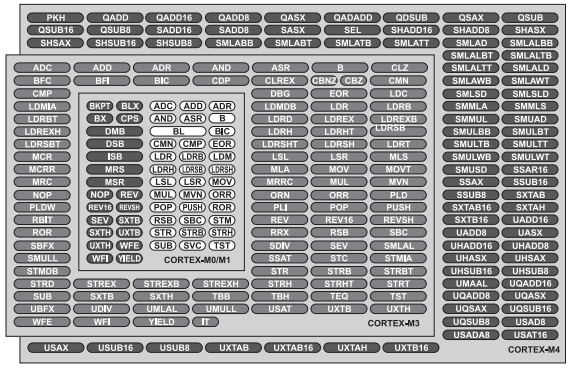
\includegraphics{rys/ARM/thumb_2}
\par\end{centering}

\caption{Rozkazy wykonywane przez rdzenie rodziny \emph{Cortex-Mx} (\emph{�r�d�o:}
\cite{Paprocki2009}) \label{fig:thumb_2}}


\end{figure}



\section{Rdze� \emph{Cortex-M3}}

\begin{figure}
\begin{centering}
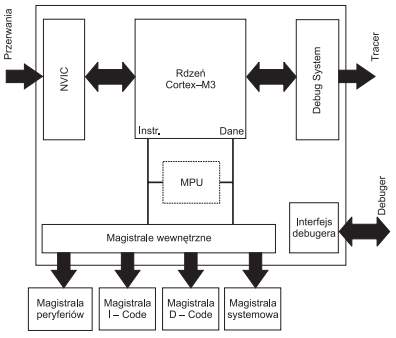
\includegraphics{rys/ARM/cortex_m3}
\par\end{centering}

\caption{Schemat rdzenia \emph{Cortex-M3} (\emph{�r�d�o:} \cite{Paprocki2009})
\label{fig:Schemat-rdzenia-Cortex-M3}}


\end{figure}


Na rysunku \ref{fig:Schemat-rdzenia-Cortex-M3} przedstawiono w spos�b
uproszczony budow� rdzenia \emph{Cortex-M3}. Obs�uguje on list� rozkaz�w
\emph{Thumb-2}, kt�ra pozwala realizowa� operacje zar�wno na liczbach
16- jak i 32-bitowych. Dzi�ki temu uzyskuje si� wi�ksz� (w por�wnaniu
do rozkaz�w \emph{ARM}) g�sto�� upakowania polece�, mniejsze zapotrzebowanie
na pami�� programu (flash) oraz szybsze wykonywanie rozkaz�w w stosunku
do programu zapisanego przy u�yciu listy \emph{Thumb}. Pisz�c program,
nie ma zatem potrzeby prze��czania si� mi�dzy 32-bitowym trybem \emph{ARM}
i 16-bitowym trybem \emph{Thumb}.

Rdze� \emph{Cortex-M3} jest zaprojektowany zgodnie z pe�n� architektur�
harwardzk�. Oznacza to rozdzielenie pami�ci programu i danych oraz
magistrali danych i rozkaz�w (rysunek \ref{fig:Architektura-Harvard}).
Zalet� takiej architektury jest mo�liwo�� dost�pu do pami�ci danych
i programu w tym samym czasie. Poniewa� jednak przestrze� adresowa
dla obu z nich jest wsp�lna, nie mog� one wykorzystywa� tej przestrzeni
w pe�ni, lecz tylko w cz�ci.

Mikrokontrolery z rdzeniem \emph{Cortex-M3} wspieraj� dost�p do danych
z uwzgl�dnieniem dw�ch sposob�w u�o�enia bajt�w, tj. \emph{little
endian} i \emph{big endian}. W pierwszym przypadku m�odsze bajty zapisywane
s� pod ni�szymi adresami, za� starsze pod wy�szymi. W przypadku big
endian jest na odwr�t. Jednak�e wyb�r sposobu u�o�enia nast�puje na
etapie produkcyjnym i jest on zapisany w jednym z rejestr�w \emph{read
only}. Odczytuj�c zawarto�� tego rejestru mo�na sprawdzi� jaki spos�b
u�o�enia bajt�w obs�ugiwany jest w danym mikroprocesorze.

Bardziej z�o�one rdzenie \emph{Cortex-M3} posiadaj� jednostk� ochrony
pami�ci MPU (ang. \emph{memory protextion unit}). Ponadto architektura
Cortex przewiduje obecno�� blok�w debugowania z obs�ug� pu�apek (ang.\emph{
breakpoint}) oraz punkt�w podgl�dowych (ang. \emph{watchpoint}).

Dla rdzeni rodziny \emph{Cortex} przewidziane s� dwa tryby pracy:
uprzywilejowany oraz u�ytkownika. W~pierwszym z nich aplikacja ma
pe�ny dost�p do wszystkich zasob�w rdzenia. Znowu� w trybie u�ytkownika,
niekt�re zasoby nie mog� by� u�ywane przez aplikacje. Takie podej�cie
pozwala na tworzenie bezpiecznych program�w, w tym system�w operacyjnych,
kt�rych j�dra pracuj� w trybie uprzywilejowanym, za� programy u�ytkownika
w trybie nieuprzywilejowanym.

\begin{figure}
\begin{centering}
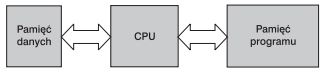
\includegraphics{rys/ARM/harvard}
\par\end{centering}

\caption{Architektura Harvard (\emph{�r�d�o: }\cite{Paprocki2009}) \label{fig:Architektura-Harvard}}


\end{figure}



\section{Rejestry og�lnego przeznaczenia}

Rdze� \emph{Cortex M3} posiada 16 rejestr�w podstawowych (R0 -- R15),
z kt�rych trzyna�cie (R0 -- R12) stanowi� rejestry og�lnego przeznaczenia
(rysunek \ref{fig:rejestry}). Wi�kszo�� rozkaz�w 16-bitowych mo�e
u�ywa� jedynie rejestr�w R0 -- R7. Rejestr R13 pe�ni funkcje wska�nika
stosu SP (ang. \emph{stack pointer}) i~w~rzeczywisto�ci sk�ada si�
z dw�ch rejestr�w bankowanych \cite{Paprocki2009}, z kt�rych w danej
chwili widoczny jest jeden:
\begin{itemize}
\item g��wnego wska�nika stosu MSP (ang. \emph{main stack pointer}) -- u�ywanego
domy�lnie przez przerwania i j�dro systemu operacyjnego pracuj�cego
w trybie uprzywilejowanym,
\item procesowego wska�nika stosu PSP (ang. \emph{process stack pointer})
-- u�ywanego przez programy u�ytkownika kontrolowane przez system
operacyjny.
\end{itemize}
Wykorzystanie dw�ch stos�w jest korzystne dla tworzenia bezpiecznych
aplikacji, gdy� uniemo�liwia dost�p do systemowego stosu, co grozi�oby
naruszeniem stabilno�ci systemu.

Pozosta�e dwa rejestry podstawowe to:
\begin{itemize}
\item R14 -- zawieraj�cy adres powrotu z podprocedury,
\item R15 -- licznik programu PC (ang. \emph{program counter}) znany te�
jako licznik instrukcji IC (ang. \emph{instruction counter}) -- zawiera
adres aktualnie wykonywanego rozkazu.
\end{itemize}
Opr�cz wymienionych rejestr�w podstawowych, rdze� \emph{Cortex-M3}
zawiera tak�e rejestry specjalne takie jak:
\begin{itemize}
\item rejestr stanu (ang. \emph{program status register}) -- zawieraj�cy
tzw. flagi,
\item rejestr maski przerwa� (ang. \emph{interrupt mask register}),
\item rejestr sterowania (ang. \emph{control register}).
\end{itemize}
Rejestry specjalne s�u�� do sterowania rdzeniem oraz do kontroli przebiegu
wykonywania programu. Mog� by� modyfikowane jedynie za pomoc� specjalnych
rozkaz�w i nie mo�e to mie� miejsca w trakcie normalnej pracy mikrokontrolera
\cite{Paprocki2009}.

\begin{figure}
\begin{centering}
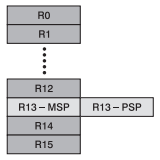
\includegraphics{rys/ARM/rejestry}
\par\end{centering}

\caption{Rejestry podstawowe rdzenia \emph{Cortex-M3} (\emph{�r�d�o:} \cite{Paprocki2009})
\label{fig:rejestry}}


\end{figure}



\section{Przestrze� adresowa}

Rdze� Cortex-M3 jest w stanie zaadresowa� przestrze� 4 GB pami�ci
\cite{Krzyzanowski207}. Obejmuje ona tzw. segmenty, m. in. pami��
programu, SRAM i zewn�trzn� pami�� RAM. Odpowiedni� map� pami�ci pokazano
na rysunku \ref{fig:Mapa-pamieci}.

\begin{figure}
\begin{centering}
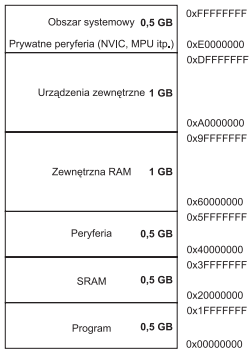
\includegraphics{rys/ARM/mapa_pamieci}
\par\end{centering}

\caption{Mapa pami�ci rdzenia \emph{Cortex-M3} (\emph{�r�d�o:} \cite{Paprocki2009})
\label{fig:Mapa-pamieci}}


\end{figure}



\section{Obszary o dost�pie bitowym}

Przestrze� adresowa rdzenia \emph{Cortex-M3} zawiera dwa obszary o
dost�pie bitowym (okre�lanych jako \emph{bit-band}): w regionie pami�ci
RAM oraz w regionie urz�dze� zewn�trznych. W pierwszym przypadku obszar
rozpoczyna si� od adresu 0x20000000, za� drugi od 0x40000000 {[}\cite{LPC1768}{]}.
Takie rozwi�zanie pozwala na optymaln� prac� rdzenia. Normalnie aby
zmieni� jeden bit, nale�y odczyta� warto�� z~w�a�ciwej kom�rki pami�ci,
ustawi� w niej warto�� odpowiedniego bitu, a nast�pnie tak zmodyfikowan�
warto�� zapisa� w pierwotnej kom�rce. Dzi�ki wykorzystaniu dost�pu
bitowego, ten sam rezultat mo�na uzyska� dzi�ki dost�powi do w�a�ciwej
kom�rki pami�ci w obszarze mapowania bit�w regionu \emph{bit-band}.
Jej odpowiedni adres mo�na wyznaczy� dzi�ki poni�szym formu�om \cite{bit_band_arm_www}:

\begin{equation}
bit\_word\_offset=(byte\_offset\cdot32)+(bit\_number\cdot4)\label{eq:bitband_formula_1}
\end{equation}


\begin{equation}
bit\_word\_addr=bit\_band\_base+bit\_word\_offset\label{eq:bitband_formula_2}
\end{equation}


gdzie:
\begin{itemize}
\item \emph{bit\_word\_offset} -- pozycja bitu w obszarze pami�ci \emph{bit-band},
\item \emph{byte\_offset} -- numer bajtu w obszarze \emph{bit-band} zawieraj�cego
��dany bit,
\item \emph{bit\_number} -- pozycja bitu w bajcie,
\item \emph{bit\_word\_addr} -- adres bajtu mapuj�cego ��dany bit w obszarze
pami�ci mapowania bit�w (\emph{alias memory region}),
\item \emph{bit\_band\_base} -- adres pocz�tku regionu mapowania bit�w (dla
obszaru pami�ci RAM wynosi on 0x22000000 \cite{Paprocki2009}).
\end{itemize}
Przyk�adowo, dla pi�tego bitu w bajcie o adresie 0x20000007, wymienione
powy�ej parametry wynosz�:
\begin{itemize}
\item \emph{bit\_number} = 5;
\item \emph{byte\_offset} = 7 (0x20000007 -- 0x20000000),
\item \emph{bit\_word\_offset} =$7\cdot32+5\cdot4=244=0x000000F4$,
\item \emph{bit\_word\_addr} = $0x22000000+0x000000F4=0x220000F4$.
\end{itemize}
Aby skasowa� lub ustawi� okre�lony bit w regionie \emph{bit-band},
nale�y wpisa� odpowiednio 0 lub 1 do w�a�ciwej kom�rki w obszarze
mapowania.

\begin{figure}
\begin{centering}
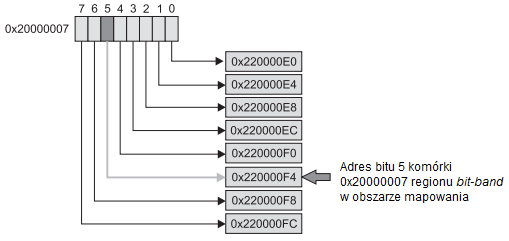
\includegraphics{rys/ARM/bit_band}
\par\end{centering}

\caption{Mapowanie pi�tego bitu kom�rki o adresie 0x20000007 z regionu bit-band
(\emph{�r�d�o:} \cite{Paprocki2009})}


\end{figure}



\section{Kontroler przerwa� \emph{NVIC}}

Aby mikroprocesor (lub centralna jednostka przetwarzaj�ca mikrokontrolera)
m�g� si� komunikowa� z urz�dzeniami peryferyjnymi poprzez uk�ady wej�cia/wyj�cia,
stosuje si� dwie techniki:
\begin{itemize}
\item przegl�danie (ang. \emph{polling}) rejestr�w uk�ad�w wej�cia/wyj�cia,
\item przerwania.
\end{itemize}
\begin{figure}
\begin{centering}
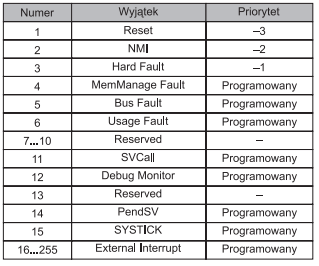
\includegraphics{rys/ARM/priorytety_przerwan}
\par\end{centering}

\caption{Przerwania obs�ugiwane przez rdze� \emph{Cortex-M3} i ich priorytety
(\emph{�r�d�o:} \cite{Paprocki2009}) \label{fig:priorytety-przerwan}}


\end{figure}


Konstrukcje dzisiejszych mikrokomputer�w s� optymalizowane pod k�tem
obs�ugi przerwa�. Rdze� \emph{Cortex-M3} posiada wbudowany kontroler
przerwa� \emph{NVIC} (ang. \emph{nested vectored interrupt controller}).
Pozwala on na obs�ug� maksymalnie pi�tnastu przerwa� (wyj�tk�w) systemowych
i 240 przerwa� zewn�trznych. Faktyczna liczba obs�ugiwanych przerwa�
zale�y od konkretnego mikrokontrolera. Wi�kszo�� przerwa� systemowych
i wszystkie przerwania zewn�trzne moga mie� ustalany programowo priorytet
\cite{Paprocki2009}. Niekt�re priorytety zgrupowano (w kolejno�ci
malej�cej) w tabeli na rysunku \ref{fig:priorytety-przerwan}. Jak
wida�, zdarzeniem o najwy�szym priorytecie w systemie jest resetowanie.

Mo�liwo�ci kontrolera \emph{NVIC} opisano skr�towo w poni�szych punktach\cite{Paprocki2009}.
\begin{enumerate}
\item Obs�uga przerwa� zagnie�d�onych (zwanych te� wielopoziomowymi) --
je�li w trakcie procedury obs�ugi przerwania ISR (ang. \emph{interrupt
service routine}) wyst�pi przerwanie o wy�szym poziomie, obs�uga bie��cego
jest przerywana, nast�puje skok do procedury obs�ugi przerwania o
wy�szym poziomie, a po jej zako�czeniu powr�t do obs�ugi zdarzenia
poprzedniego (rysunek \ref{fig:wielpoz-obsluga-przerwan}).
\item Sprz�towa obs�uga wektor�w przerwa� -- adres funkcji obs�ugi przerwania
jest pobierany z wektora w pami�ci i nie ma potrzeby jego programowego
wyznaczania, dzi�ki czemu czas obs�ugi zdarzenia jest mniejszy.
\item Dynamiczna zmiana priorytet�w przerwa� -- pozwala zmienia� programowo
priorytet przerwania podczas wykonywania programu. Nie mo�na jednak
zmieni� priorytetu przerwania przed wyj�ciem z procedury jego obs�ugi,
dzi�ki czemu unika si� sytuacji wielokrotnego obs�u�enia tego samego
zdarzenia podczas zmiany priorytetu.
\item Zoptymalizowane op�nienia czasowe obs�ugi przerwa� -- uzyskano to
m. in. dzi�ki automatycznemu zapisywaniu i odzyskiwaniu tzw. kontekstu
zadania, a wi�c zawarto�ci najwa�niejszych dla niego rejestr�w. Inne
sposoby skr�cenia op�nie� w obs�udze przerwa� (np. \emph{Tail-Chaining},
przerywanie operacji POP) opisano w literaturze \cite{Paprocki2009}.
\item Maskowanie przerwa� - przerwania mog� by� maskowane na podstawie wysoko�ci
priorytet�w lub maskowane ca�kowicie poprzez wpisy do w�a�ciwych rejestr�w
maskuj�cych.
\end{enumerate}
\begin{figure}
\begin{centering}
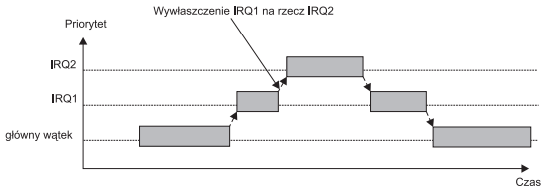
\includegraphics{rys/ARM/przerwania_zagniezdzone}
\par\end{centering}

\caption{Wielopoziomowa obs�uga przerwa� (\emph{�r�d�o: }\cite{Paprocki2009})
\label{fig:wielpoz-obsluga-przerwan}}


\end{figure}



\section{Lista instrukcji \emph{Thumb-2}}

Jedn� z najwi�kszych zalet rdzenia \emph{Cortex-M3} z punktu widzenia
programisty, jest mo�liwo�� wykorzystania rozkaz�w operuj�cych na
danych 16- i 32-bitowych bez konieczno�ci dodatkowych zabieg�w (prze��czanie
si� mi�dzy trybami). Dzi�ki temu uzyskuje si� zmniejszenie zu�ycia
pami�ci programu przy jednoczesnym wzro�cie szybko�ci jego wykonywania
\cite{Paprocki2009}.

W celu jeszcze lepszego wykorzystania ww. cech rdzenia \emph{Cortex-M3},
stworzono odmian� asemblera oznaczan� w skr�cie jako UAL (ang. \emph{unified
assembly language}). Pozwala ona w �atwiejszy i czytelniejszy spos�b
wykorzystywa� w programie rozkazy 16- i 32-bitowe.

Zestaw rozkaz�w \emph{Thumb-2} zawiera operacje, kt�re mog� by� wykonywane
zar�wno jako 16- jak i~32-bitowe. O rodzaju operacji decyduje przyrostek
(\emph{N} dla instrukcji 16-bitowych, \emph{W} dla 32-bitowych) dodawany
po kropce do w�a�ciwego mnemonika instrukcji (np. \emph{ADDS.N} lub
\emph{ADDS.W}, gdzie \emph{ADDS} jest instrukcj� dodawania liczby
do zawarto�ci rejestru b�d�cego operandem). Mnemoniki pozbawione sufiksu
s� zwykle t�umaczone na instrukcje 16-bitowe.

Jak wida� programowanie rdzenia \emph{Cortex-M3} w j�zyku asemblera
niesie ze sob� spore mo�liwo�ci optymalizacji. Wad� tak niskopoziomowego
podej�cia jest czasoch�onno��, du�y nak�ad pracy i cz�sto tak�e kiepska
czytelno�� kodu. Decyzje o pisaniu aplikacji (b�d� jej fragment�w)
w asemblerze powinny by� wynikiem kompromisu mi�dzy wzgl�dami wydajno�ciowymi
oraz ekonomicznymi.

\chapter{Pomiar}


\section{Uk�ady elektroniczne}

Wyznaczenie pozycji w przestrzeni wymaga�o harmonijnego wsp�dzia�ania
trzech zastosowanych w niniejszej pracy uk�ad�w elektronicznych. Najwa�niejszym
elementem, by� zestaw uruchomieniowy LandTiger, zawieraj�cy mikrokontroler
LPC1768 opartym o rdze� ARM Cortex-M3. Mikrokontroler odpowiada� za
odczyt, przetwarzanie i przesy�anie danych pomiarowych zgromadzonych
przez dwa urz�dzenia firmy Digilent: PmodACL i PmodGYRO. Pierwszy
z tych uk�ad�w to tr�josiowy, cyfrowy akcelerometr pracuj�cy na akcelerometrze
ADXL345 firmy AnalogDevices. PmodGYRO oparty jest na uk�adzie L3G4200D
firmy ST Microelectronics.

ADXL345 to niewielki akcelerometr posiadaj�cy wysok� rodzielczo��
wykonywanych pomiar�w (13-bit�w) i wykonuj�cy pomiary w zakresie \textpm{}16g.
Urz�dzenie to dokonuje pomiaru zar�wno dynamicznego przy�pieszenia
b�d�cego rezultatem ruchu, jak r�wnie� przy�pieszenia statyczne takie
jak grawitacja, kt�ra pozwalaj� pracowa� jako czujniki przeci��enia.
Czujnik ten jest przy�pieszeniomerzem pojemno�ciowym, kt�rego zasada
dzia�ania zosta�a ju� opisana wcze�niej.

L3G4200D to tr�josiowy czujnik przy�pieszenia k�towego o rozdzielczo�ci
16 bit�w, zapewniaj�cy niewielki dryft zera oraz wysok� czu�o��, niezale�n�
od czasu i temperatury. Uk�ad ten posiada trzy zakresy pomiarowowe:
\textpm{}250/\textpm{}500/\textpm{}2000 dps oraz jest zdolny do wykonywania
pomiar�w w pa�mie wybranym przez u�ytkownika. �yroskopy firmy ST Microelectronics
maj� lepsz� stabilno�� i czu�o�� w funkcji temperatury oraz odporno�ci
na uszkodzenia mechaniczne. Przewaga wynika z innego sposobu monta�u
struktury uk�adu pomiarowego. W zastosowanym urz�dzeniu, jest on zamontowany
w jednym, centralnym punkcie, zamiast w kilku, jak ma to miejsce w
innych rozwi�zaniach. Dzi�ki temu si�y wynikaj�ce ze zmian temperatury,
napr�e� mechanicznych przenosz� si� na uk�ad pomiarowy w znacznie
miejszym stopniu. Dodatkowo wykorzystany �yroskop bazuje na jednej
masie pomiarowej dla wszystkich trzech osi, co znacz�co poprawia symetri�
sygna��w wyj�ciowych i skutkuje mniejszymi rezonansami.


\section{Po��czenie uk�ad�w}

Posiadaj�c trzy osobne uk�ady wymienione w poprzednim paragrafie,
konieczne by�o odpowiednie po��czenie ich ze sob�. Wykonano w tym
celu p�ytk�, w kt�rej zamontowano gniazdo 34-pinowe, dwurz�dowe �e�skie
i dwa z��cza k�towe dwurz�dowe 12-pinowe. Schemat wykonanego uk�adu
przedstawiono na rysunku:

\begin{figure}
\begin{centering}
\includegraphics[scale=0.6]{rys/p�ytka}
\par\end{centering}

\caption{Schemat po��czenia mikrokontrolera z urz�dzeniami pomiarowymi}
\end{figure}


Przedstawiony na rysunku schemat przygotowano na zwyk�ej p�ytce uniwersalnej.
Do po��czenia z zestawem uruchomieniowym wykorzystano z��cze 34-pinowe
s�u��ce domy�lnie do po��czenia z ekranem LCD. Zawiera�o ono wszystkie
piny konieczne do zapewnienia poprawnej pracy obu urz�dze� pomiarowych.
Dodatkowo na p�ytce zamontowano dwa z��cza 12-pinowe, do kt�rych wpi�to
uk�ady PmodACL i PmodGYRO. Wykorzystanie wspomnianego z��cza z zestawu
uruchmieniowego pozwala�o na stabilne przy��czenie akcelerometra i
�yroskopu. Dzi�ki takiemu rozwi�zaniu, pomiar dotyczy ca�ego uk�adu
LandTiger zapewniaj�c niezawodno�� po��czenia pomi�dzy wszystkimi
p�ytkami drukowanymi wchodz�cymi w sk�ad zestawu pomiarowego.




\section{Komunikacja}

Ostatnim elementem pomiaru, kt�ry obs�ugiwany jest przez mikroprocesor
jest wys�anie zmierzonych danych do komputera. W tym celu wybrano
interfejs UART, kt�ry umo�liwia asynchroniczne odbieranie i nadawnie
unformacji przy pomocy portu szeregowego (opisany w rozdziale 4.3).
Odbi�r i dalsze przetwarzanie nast�powa�o w komputerze przeno�nym,
niewyposa�onym w z��cze szeregowe. Z tego wzgl�du konieczne by�o zakupienie
konwertera RS-232 na USB. Wykorzystano w tym celu przej�ci�wk� opart�
na chipsecie PL2303HX. Po zainstalowaniu odpowiednich sterownik�w,
port COM stawa� si� widoczny w systemie. Dzi�ki temu mo�liwe by�o
odbieranie danych pomiarowych, przeliczenie i wy�wietlanie ich w aplikacji.

W nieniejszej pracy wykorzystano wysy�anie i odbieranie danych za
po�rednictwem interfejsu UART. Zar�wno wysy�anie, jak i odbieranie
danych oparto na przerwaniach. Przerwania by�y generowane w momencie
pojawienia si� danych b�d� to w buforze wej�ciowym, b�d� te� w buforze
wyj�ciowym. Oba te typy by�y obs�ugiwane przez jedn� procedur� obs�ugi
przerwania. W zale�no�ci od typu bufora, kt�ry otrzyma� dane, przeprowadzano
odczyt lub zapis danych. Mikroprocesor otrzymywa� z komputera tylko
jeden typ danych: by� to ci�g tekstowy ``RESET''. Po jego otrzymaniu
nast�powa�o wyzerowanie zmiennych przechowuj�cych wyniki dotychczasowych
pomiar�w k�ta obrotu i przyspieszenia. Poprzez interfejs UART wysy�ano
�a�cuchy znakowe zawieraj�ce wyniki. Dane pomiarowe by�y zapisywane
w postaci C-stringa sk�adaj�cego si� z sze�ciu liczb ca�kowitych oddzielonych
znakami spacji. Trzy pierwsze liczby by�y wynikami odczytanymi z akcelerometru
dla osi X, Y i Z, a trzy kolejne to dane z �yroskopu dla ka�dej z
osi. Tak przygotowany �a�cuch przesy�any by� do komputera, gdzie nast�powa�a
jego obr�bka maj�ca na celu uzyskanie warto�ci liczbowych.

\chapter{Interfejs u�ytkownika}

W poprzednim rozdziale opisano wszystkie dzia�ania, kt�re podj�to
w celu dokonania pomiaru przemieszczenia i k�ta obrotu uk�adu. Dane
przes�ane do komputera nie mog� by� jedynie wy�wietlone po stronie
komputera w postaci ci�gu znak�w, gdy� to praktycznie uniemo�liwia�oby
analiz� otrzymywanych danych. Z tego wzgl�du konieczne jest odpowiednie
przekszta�cenie otrzymanych danych w spos�b, kt�ry umo�liwi zobrazowanie
zmierzonych przemieszcze� b�d� obrot�w. W tym celu przygotowano aplikacj�,
kt�rej zadaniem jest odbi�r i wy�wietlenie wynik�w w formie graficznej.
Wykorzystano do tego platform� .NET i j�zyk C\# z wykorzystaniem \emph{Windows
Forms} dla stworzenia interfejsu. Powodem wyboru tej technologii by�a
wzgl�dna prostota oraz mnogo�� klas i technik, kt�re umo�liwia�y osi�gni�cie
postawionego celu na systemie Windows. 


\section{Okno g��wne aplikacji}

Okno g��wne zrealizowanego programu przedstawiono na rysunku \ref{fig:Okno-g=000142=0000F3wne-programu}.

\begin{figure}
\begin{centering}
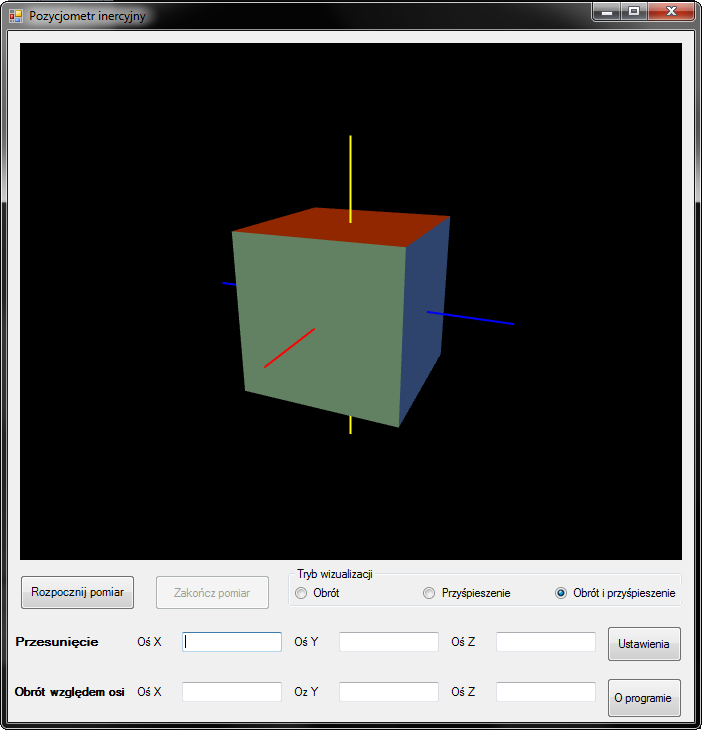
\includegraphics[scale=0.6]{rys/aplikacja/okno_glowne}
\par\end{centering}

\caption{Okno g��wne programu\label{fig:Okno-g=000142=0000F3wne-programu}}
\end{figure}


Otrzymane wyniki pomiaru przemieszczenia i k�ta obrotu wypisane s�
w odpowiednich polach, dla ka�dej z osi osobno. Jednak�e najwa�niejszym
elementem aplikacji jest okno wy�wietlania wynik�w pomiaru w formie
graficznej. Sze�cian symbolizuje uk�ad pomiarowy, dodatkowo przedstawiono
osie uk�adu wsp�rz�dnych: o� X jest koloru niebieskiego, o� Y - czerwonego
a o� Z jest ��ta. Dzi�ki temu mo�na �atwiej zaobserwowa� wszelkie
przemieszczenia i zmiany k�ta wzgl�dem po�o�enia pocz�tkowego. Poni�ej
okna wizualizacji umieszczono trzy prze��czniki zgrupowane w panelu
\emph{Tryb pomiaru}. Umo�liwiaj� one prze��czanie si� pomi�dzy trzema
r�nymi trybami wizualizacji. \emph{Obr�t} umo�liwia obserwacj� jedynie
wynik�w pracy �yroskopu, \emph{Przemieszczenie} wy��cza wizualizacj�
obrot�w bry�y pozostawiaj�c tylko przemieszczenie, a ostatni prze��cznik
pozwala na pe�ny podgl�d wynik�w pomiar�w. Przycisk \emph{Ustawienia}
pozwala na zmian� parametr�w po��czenia w osobnym oknie. Zostanie
ono szczeg�owo opisane w kolejnej cz�ci. Wci�ni�cie przycisku \emph{O
programie} wy�wietla informacj� o zrealizowanej pracy in�ynierskiej
(rysunek \ref{fig:Okno-informacji-o-programie}). 

\begin{figure}
\centering{}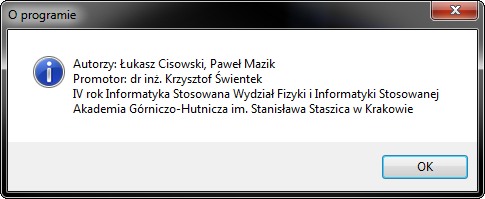
\includegraphics[scale=0.7]{rys/aplikacja/info}\caption{Okno informacji o programie\label{fig:Okno-informacji-o-programie}}
\end{figure}


Za rozpocz�cie i zako�czenie pomiar�w odpowiadaj� przyciski \emph{Rozpocznij
pomiar} i\emph{ Zako�cz pomiar}. W danej chwili tylko jeden z przycisk�w
jest aktywny, dzi�ki czemu nie ma mo�liwo�ci wielokrotnego zainicjalizowania/zako�czenia
po��czenia z wykorzystaniem interfejsu szeregowego. W przypadku pr�by
nawi�zania po��czenia bez odpowiednio skonfigurowanych parametr�w
po��czenia wy�wietlony zostanie odpowiedni komunikat informuj�cy o
konieczno�ci poprawienia wprowadzonych danych (rysunek \ref{fig:Okno-b=000142=000119du-po=000142=000105czenia}).

\begin{figure}
\begin{centering}
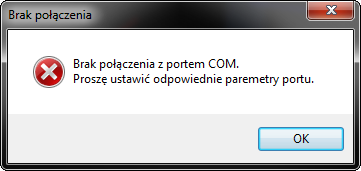
\includegraphics[scale=0.7]{rys/aplikacja/blad}\caption{Okno b��du po��czenia z portem COM\label{fig:Okno-b=000142=000119du-po=000142=000105czenia}}

\par\end{centering}

\end{figure}



\section{Okno ustawie�}

Okno ustawie� parametr�w transmisji szeregowej przedstawiono na ilustracji
\ref{fig:Opcje-programu}.

\begin{figure}
\begin{centering}
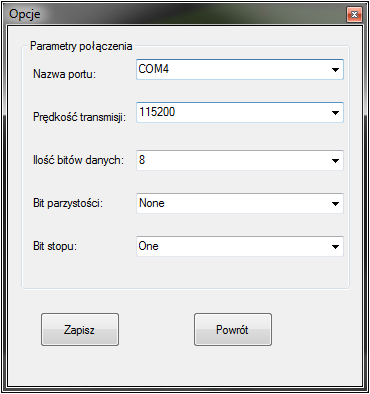
\includegraphics[scale=0.7]{rys/aplikacja/opcje}\caption{Opcje programu\label{fig:Opcje-programu}}

\par\end{centering}

\end{figure}


Kluczow� klas�, kt�ra s�u�y do przechowywania parametr�w po��czenia
dost�pnych i wybranych jest klasa statyczna \texttt{CommunicationParameters}.
Klasa ta zapami�tuje wybrane parametry transmisji danych i tablice
danych wy�wietlanych w listach rozwijanych. Nazwy port�w szeregowych
dost�pnych w danym komputerze otrzymano korzystaj�c z metody \texttt{GetPortNames()}
klasy \texttt{SerialPort} znajduj�cej si� w przestrzeni nazw \emph{System.Port.IO},
wykorzystywanej w aplikacji do komunikacji z mikroprocesorem. Aby
rozpocz�� pomiar konieczne jest jedynie wybranie odpowiedniej nazwy
portu. Reszta parametr�w domy�lnie ustawiona jest na warto�ci, kt�re
wybrano ju� w momencie konfiguracji komunikacji poprzez interfejs
UART w mikroprocesorze. W przypadku zmiany tych parametr�w, konieczne
jest wybranie odpowiednich warto�ci w oknie opcji. Klikni�cie przycisku\emph{
Zapisz} powoduje zapami�tanie wybranych parametr�w i powr�t do okna
g��wnego.


\section{Komunikacja z portem szeregowym}

Pierwszym zadaniem by�o odebranie danych pomiarowych otrzymanych z
mikroprocesora za po�rednictwem portu szeregowego. Za komunikacj�
z tym portem odpowiedzialna jest klasa \texttt{COMPortManager}. W
ramach tej klasy wykorzystano klas� biblioteczn� \texttt{SerialPort},
o kt�rej wspomniano ju� wcze�niej. Klasa ta umo�liwia kontrol� port�w
szeregowych komputera. Zapewnia ona komunikacj� synchroniczn�, sterowan�
zdarzeniami wspieraj�c� szereg typ�w kodowania: ASCII, UTF8, Unicode
i UTF32. 

Komunikacja z portem szeregowym odbywa si� w puli w�tk�w, dzi�ki czemu
wykonywana jest ona w tle. W przypadku, gdy za pomoc� tego portu otrzymane
zostan� dane, wywo�ywane jest zdarzenie obs�ugiwane przez metod� \texttt{SerialPortDataRecieved()}.
Odczytuje ona dane otrzymane z portu szeregowego i zapisuje je w postaci
stringu. Nast�pnie dane te s� opakowywane w klas� \texttt{ReceivedDataEventArgs},
kt�ra odpowiada za przechowywanie danych zdarzenia. Potem wywo�ywane
jest zdarzenie z uzyskanymi wynikami, kt�re przekazuje je do g��wnego
okna aplikacji. W klasie \texttt{COMPortManager} jest r�wnie� zaimplementowana
metoda, kt�rej zadaniem jest wysy�anie do mikroprocesora komunikatu
o tre�ci ,,RESET'', kt�ry powoduje wyzerowanie dotychczasowych wynik�w
pomiar�w.


\section{Przeliczenie otrzymanych wynik�w}

Klasa \texttt{ApplicationWindow}, wy�wietlaj�ca g��wne okno aplikacji,
odbiera dane z klasy \texttt{COMPortManager} w procedurze obs�ugi
zdarzenia. Dodatkowo metoda ta rozpoczyna si� od sprawdzenia, czy
wywo�ywanie nie jest wykonywane spoza g��wnego w�tku. Je�li taka sytuacja
ma miejsce, metoda ta zapisywana jest jako delegat, kt�ry zostaje
wykonany asynchronicznie z argumentami otrzymanymi z klasy obs�uguj�cej
komunikacj� z portem szeregowym. 

String zawieraj�cy wyniki odczytane z akcelerometru i �yroskopu zostaje
nast�pnie rozdzielony na poszczeg�lne dane. Trzy pierwsze elementy
zawieraj� u�rednione przyspieszenia, kolejne trzy to �rednie pr�dko�ci
zmierzone przez �yroskop. Zostaj� one zapisane do dw�ch tablic �a�cuch�w
znakowych, a~nast�pnie przekszta�cone do postaci liczb ca�kowitych,
kt�re pos�u�� do dalszych przelicze�.

W celu wyznaczenia przemieszcze� na podstawie uzyskanych przyspiesze�,
nale�y dokona� ich dwukrotnego ca�kowania (\cite{acl_integrating}).
W tym celu wykorzystano metod� trapez�w, znan� tak�e jako metoda Tustina.
Jest to metoda numeryczna, polegaj�ca na zast�pieniu krzywej ci�g�ej
(w tym wypadku przebiegu przyspieszenia) �aman� sk�adaj�c� si� z odcink�w
��cz�cych kolejne pr�bki pomiarowe. Pole pod krzyw� (ca�ka oznaczona)
przybli�a si� polem pod �aman�. Korzystaj�c z tej metody, mo�na wyznaczy�
sk�adow� pr�dko�ci w osi X w nast�puj�cy spos�b (\cite{acl_integrating}):

\begin{equation}
v_{x}^{n+1}=v_{x}^{n}+\left[a_{x}^{n}+\left(\frac{a_{x}^{n+1}-a_{x}^{n}}{2}\right)\right]\Delta t,\label{eq:metoda_trapezow}
\end{equation}


gdzie
\begin{itemize}
\item $v_{x}^{n}$-- warto�� pr�dko�ci w osi \emph{X} w \emph{n}-tym kroku
obliczeniowym,
\item $a_{x}^{n}$-- warto�� przyspieszenia w osi \emph{X} w \emph{n}-tym
kroku obliczeniowym,
\item $\Delta t$ -- krok ca�kowania (w tym wypadku okres pr�bkowania).
\end{itemize}
Analogicznie wyznacza si� pr�dko�ci i po�o�enia w pozosta�ych osiach.

W celu wyeliminowania wp�ywu szum�w przy braku przyspieszenia, okre�lono
warto�ci progowe (rysunek \ref{fig:discrimination_win}), kt�re uznawane
s� za zak��cenia (\cite{acl_integrating}).

\begin{figure}
\begin{centering}
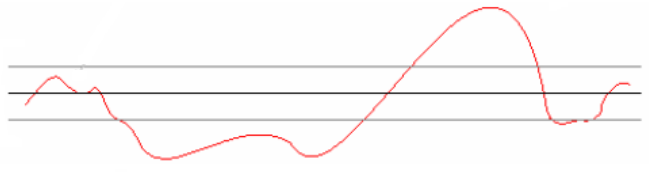
\includegraphics{rys/obliczenia/discrimination_window}
\par\end{centering}

\caption{Eliminacja szum�w przy braku przyspieszenia (\emph{�r�d�o:} \cite{acl_integrating})\label{fig:discrimination_win}}


\end{figure}




Pami�taj�c, �e akcelerometr nie mierzy przyspieszenia w $\frac{m}{s^{2}}$,
lecz w surowych liczbach (ang. \emph{raw data}), nale�a�o dokona�
przeliczenia jednostek bior�c pod uwag� czu�o�� sensora.

Analogicznie post�piono ca�kuj�c pr�dko�ci k�towe mierzone przez �yroskop
w celu obliczenia k�t�w. Jak zosta�o wcze�niej powiedziane, pomiar
taki obarczony jest b��dem zwi�zanym z dryftem i eliminuje si� go
poprzez uwzgl�dnienie pomiaru k�ta akcelerometrem. Og�lnie mo�na zapisa�,
�e

\begin{equation}
\alpha=k\alpha_{g}+\left(1-k\right)\alpha_{a},\label{eq:filtr_komplementarny}
\end{equation}


gdzie
\begin{itemize}
\item $\alpha_{g}$-- k�t obliczony przy pomocy danych pomiarowych z �yroskopu,
\item $\alpha_{a}$-- k�t obliczony przy pomocy danych pomiarowych z akcelerometru,
\item \emph{k} -- wsp�czynnik z przedzia�u (0 - 1).
\end{itemize}
Zale�no�� \ref{eq:filtr_komplementarny} wyra�a znan� w literaturze
z dziedziny przetwarzania sygna��w filtracj� komplementarn�. W omawianym
przypadku pozwala ona zniwelowa� b��d dryftu zwi�zany z �yroskopem
oraz b��d pomiaru k�ta przy pomocy akcelerometru, wynikaj�cy z obecno�ci
przyspiesze� innych ni� grawitacyjne. Mo�na powiedzie� r�wnie�, �e
podana metoda ��czy zalety pomiar�w �yroskopem i akcelerometrem. Wsp�czynnik
\emph{k} dobiera si� empirycznie. Dok�adniejsze wyniki, lecz du�o
bardzie z�o�one obliczeniowo, daje filtracja Kallmana, szeroko opisywana
w publikacjach z dziedziny przetwarzania sygna��w. W metodzie tej,
wagi z jakimi brane s� wielko�ci pochodz�ce od poszczeg�lnych czujnik�w
obliczane s� na bie��co.

\begin{figure}
\begin{centering}
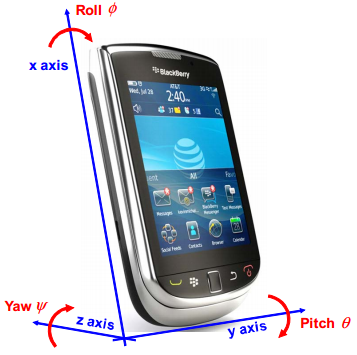
\includegraphics{rys/obliczenia/rpy}
\par\end{centering}

\caption{K�ty \emph{roll}, \emph{pitch} i \emph{yaw} (\emph{�r�d�o:} \cite{RPY})\label{fig:katy_rpy}}


\end{figure}


W celu wyznaczenia k�t�w (rys. \ref{fig:katy_rpy}) $\phi$ oraz $\theta$
przy pomocy danych pochodz�cych z akcelerometru, mo�na pos�u�y� si�
nast�puj�cymi zale�no�ciami (\cite{RPY}):

\begin{equation}
tan\left(\phi\right)=\frac{a_{y}}{a_{z}},\label{eq:roll_equation}
\end{equation}


\begin{equation}
tan\left(\theta\right)=\frac{-a_{x}}{\sqrt{a_{z}^{2}+a_{y}^{2}}},\label{eq:pitch_equation}
\end{equation}


gdzie \emph{a\textsubscript{x}}, \emph{a\textsubscript{y}}, \emph{a\textsubscript{z}}
s� przyspieszeniami (w naszym przypadku u�rednionymi przyspieszeniami)
odpowiednio w osi X, Y i Z.

Jak wida�, wz�r \ref{eq:pitch_equation} nie pozwala na poprawne okre�lenie
�wiartki uk�adu wsp�rz�dnych, w kt�rej znajduje si� mierzony k�t.
Ponadto je�li sk�adowe przyspieszenia w osiach Y i Z b�d� r�wne zeru,
niemo�liwe b�dzie okre�lenie k�ta obrotu wok� osi X. Ma to proste
uzasadnienie fizyczne -- sk�adowe \emph{a\textsubscript{\emph{y}}}
i \emph{a\textsubscript{\emph{z}}} b�d� r�wne jednocze�nie zeru,
gdy o� X b�dzie r�wnoleg�a do wektora grawitacji. W�wczas obr�t wok�
osi X jest ,,niewidoczny'' dla akcelerometru, gdy� nie rejestruje
on �adnych zmian przyspieszenia we wszystkich osiach.

W celu wyznaczenia k�ta $\psi$ nale�y zastosowa� magnetometr (\cite{RPY},
\cite{RPY_compas}). Jest to przyrz�d potrafi�cy mierzy� warto�� ziemskiego
pola magnetycznego. Je�li umie�cimy kompas tak, by jego p�aszczyzna
XY by�a r�wnoleg�a do powierzchni ziemi, to obracanie nim wok� osi
Z spowoduje, �e b�dzie rejestrowa� r�ne warto�ci pola magnetycznego
w osiach X i Y. Sk�adowe te mog� pos�u�y� do oszacowania kata obrotu.

Otrzymane wyniki zapisywane s� do odpowiednich p�l tekstowych w oknie
g��wnym aplikacji. Ze wzgl�du na fakt, i� wyliczone warto�ci nie mog�
by� bezpo�rednio zapisane do klasy dzia�aj�cej w innym w�tku, konieczne
by�o zastosowanie metody \texttt{Invoke()} klasy \texttt{Dispatcher}
na obiekcie okna wizualizacji. Klasa \texttt{Dispatcher} umo�liwia
zarz�dzenia kolejk� element�w roboczych dla danego w�tku, w tym wypadku
okna wizualizacji. Metoda \texttt{Invoke()} jako argument przyjmuje
delegat do funkcji, kt�ra zostanie na tym w�tku wykonana. T� funkcj�
jest metoda klasy \texttt{ApplicationWindow} o nazwie \texttt{ApplyMovement()},
kt�ra jako argumenty przyjmuje dwie tablice danych z wynikami z obu
urz�dze� pomiarowych. Warto�ci te s� przypisywane do odpowiednich
zmiennych. Nale�y tutaj zaznaczy�, �e w~przypadku, gdy metoda ta
wywo�ywana jest po raz pierwszy, wyniki pomiaru przesuni�cia/obrotu
s� bezpo�rednio wpisywane do odpowiednich zmiennych w obiekcie okna
wizualizacji, a ich warto�ci zapami�tywane w odpowiedniej zmiennej
w klasie \texttt{ApplicationWindow}. Ka�dy kolejny pomiar skutkuje
zapisaniem do okna liczby b�d�cej r�nic� poprzedniej i obecnej. Dzi�ki
temu, aktualizacja pozycji sze�cianu skutkuje jego przesuni�ciem jedynie
o warto�� b�d�c� r�nic� pomi�dzy dwoma kolejnymi pomiarami. Po zapisaniu
warto�ci zmiennych, wywo�ywana jest w oknie metoda, kt�rej zadaniem
jest wykonanie wszystkich transformacji na sze�cianie. 

Metoda powoduj�ca usuni�cie wszystkich transformacji r�wnie� jest
wywo�ywana z wykorzystaniem metody \texttt{Invoke()} klasy \texttt{Dispatcher}.
Dzi�ki niej mo�na przywr�ci� domy�lne po�o�enie sze�cianu i rozpocz��
pomiar od pocz�tku, okre�laj�c bie��ce po�o�enie uk�adu jako domy�lne.
Metoda ta jest wywo�ywana ka�dorazowo przy prze��czaniu trybu wizualizacji,
jak r�wnie� po zako�czeniu pomiaru.


\section{Wizualizacja danych}

Bior�c pod uwag� za�o�enia przyj�te przed realizacj� pracy, by� to
najwa�niejszy etap w tworzeniu interfejsu u�ytkownika. Konieczny by�
wyb�r takiej technologii, kt�ra dobrze wsp�gra�a z reszt� programu
napisan� w j�zyku C\#, a jednocze�nie zapewnia�aby du�e mo�liwo�ci
wizualizacji danych w postaci obiekt�w tr�jwymiarowych. Z tego wzgl�du
zdecydowano si� skorzysta� z \emph{Windows Presentation Foundation}.
Jest to silnik graficzny oparty o grafik� wektorow�, kt�ry daje du�e
mo�liwo�ci tworzenia aplikacji. API w WPF opiera si� na j�zyku XML,
a dok�adniej wykorzystuje jego implementacj� o~nazwie XAML. Zapewnia
on powi�zanie pomi�dzy interfejsem a logik� i umo�liwia tworzenie
zaawansowanych kontrolek, grafiki 2D i 3D, animacji, dokument�w, multimedi�w
czy te� tekstu. Dodatkow� zalet� jest fakt, i� \emph{Windows Presentation
Foundation} jest zawarta w Microsoft .NET Framework, co czyni j� �atwo
dost�pn� i zdoln� do pracy z innymi elementami biblioteki .NET Framework.

Okno wizualizacji zbudowane zosta�o jako biblioteka ��czona dynamicznie.
Takie rozwi�zanie jest konieczne ze wzgl�du na fakt, i� okno stworzone
w WPF b�dzie umieszczone w interfejsie stworzonym za pomoc� \emph{Windows
Forms}. Dodatkowo konieczne by�o pod��czenie kilku bibliotek, kt�re
s� niezb�dne w poprawnym dzia�aniu aplikacji. 

Podstawowym elementem tworz�cym grafik� 3D jest tr�jk�t. Stworzenie
za pomoc� tr�jk�t�w sze�cianu nie jest szczeg�lnie trudnym wyzwaniem.
Problemem okaza�o si� narysowanie za pomoc� tr�jk�ta linii, kt�re
oznacza�y osie uk�adu wsp�rz�dnych. Teoretycznie lini� mo�na narysowa�
z wykorzystaniem odpowiednio przeskalowanego prostok�ta, lecz w takim
wypadku pojawia si� problem z zapewnieniem odpowiedniego o�wietlenia
i ustawienia kamery. Ze wzgl�du na znaczne trudno�ci, jakie mog�a
nie�� ze sob� implementacja tego rozwi�zania, zdecydowano si� na wykorzystanie
biblioteki \emph{3DTools} przygotowanej przez Microsoft. Zawiera ona
klas� \texttt{ScreenSpaceLines3D}, kt�re pozwalaj� na proste kre�lenie
linii.

Jak ju� wspomniano w poprzednim paragrafie, dwie metody klasy \texttt{ApplicationWindow}
operuj� bezpo�rednio na danych klasy \texttt{MainWindow}, odpowiadaj�cej
za wizualizacj� wynik�w pomiaru. Najwa�niejsz� z metod w tej klasie
jest metoda \texttt{ApplyTransformation()}, kt�ra na podstawie danych
zapisanych przez metod� \texttt{ApplyMovement()} z interfejsu wykonuje
odpowiednie transformacje na sze�cianie. W tym celu wykorzystywane
s� dwie klasy: \texttt{AxisAngleRotation3D} i~\texttt{TranslateTransform3D}.
Klasa \texttt{AxisAngleRotation3D} s�u�y do obracania danego obiektu.
Do jej poprawnej pracy konieczne jest podanie osi obrotu i k�ta, o
jaki nale�y obr�ci� obiekt. \texttt{TranslateTransform3D} przesuwa
obiekt o dany wektor. Wsp�rz�dne tego wektora to warto�ci otrzymane
z akcelerometru. Tak przygotowane obiekty tych klas dodaje si� do
kolekcji transformacji przypisanych do obiektu, w tym przypadku sze�cianu.

Powr�t do stanu pocz�tkowego realizowany jest w metodzie \texttt{RemoveAllTransformations}.
Odczytywana jest kolekcja transformacji, kt�re wykonano na obiekcie,
a nast�pnie s� one usuwane w kolejno�ci odwrotnej do dodania. Dzi�ki
temu mamy pewno��, �e wszystkie przesuni�cia i obroty zostan� poprawnie
usuni�te i obiekt powr�ci do domy�lnego po�o�enia. Niestety w wyniku
kolejkowania danych otrzymanych z mikroprocesora mo�e doj�� do sytuacji,
gdy po usuni�ciu wszystkich transformacji, dane otrzymane po resecie
spowoduj� przesuni�cie sze�cianu. Jednak�e warto�ci te nie wp�ywaj�
znacz�co na pogorszenie jako�ci otrzymanych wynik�w.

\nocite{3Dtools,draw_cube,net_class_library,serial_port,transformations,uart_interupt,wpf3D_in_wf,wpf_in_wf}\nocite{wpf_lines}


\bibliography{bibliografia}


\appendix

\chapter*{Dodatek A}

Tu, trzeba zamieszcza� tre�� dodatkow� np. fragmenty kodu aplikacji
itp.

\end{document}
